\documentclass[11pt]{article}
\ifdefined\pdfinfoomitdate\pdfinfoomitdate=1\fi
\ifdefined\pdftrailerid\pdftrailerid{}\fi
\ifdefined\pdfsuppressptexinfo\pdfsuppressptexinfo=15\fi
\usepackage[T1]{fontenc}
\usepackage{lmodern}
\usepackage[margin=1in]{geometry}
\usepackage{amsmath,amssymb,amsthm,mathtools}
\usepackage{microtype}
\usepackage{enumitem,booktabs}
\usepackage{xcolor,tikz}
\usetikzlibrary{arrows.meta,positioning,calc,decorations.pathreplacing,matrix,fit}
\usepackage[numbers,sort&compress]{natbib}
\usepackage[hyphens]{url}
\usepackage{hyperref}
\hypersetup{colorlinks=true,linkcolor=blue!45!black,citecolor=blue!45!black,
 urlcolor=blue!45!black,pdfauthor={OpenAI},
 pdftitle={A Power Saving for Polynomial Differences at Prime Arguments}}
\newtheorem{theorem}{Theorem}[section]
\newtheorem{proposition}[theorem]{Proposition}
\newtheorem{lemma}[theorem]{Lemma}
\newtheorem{corollary}[theorem]{Corollary}
\theoremstyle{definition}
\newtheorem{definition}[theorem]{Definition}
\theoremstyle{remark}
\newtheorem{remark}[theorem]{Remark}
\numberwithin{equation}{section}
\newcommand{\R}{\mathbb R}
\newcommand{\C}{\mathbb C}
\newcommand{\N}{\mathbb N}
\newcommand{\Z}{\mathbb Z}
\newcommand{\Q}{\mathbb Q}
\newcommand{\F}{\mathbb F}
\newcommand{\E}{\mathbb E}
\newcommand{\Prb}{\mathbb P}
\newcommand{\1}{\mathbf 1}
\newcommand{\eps}{\varepsilon}
\newcommand{\norm}[1]{\lVert#1\rVert}
\newcommand{\abs}[1]{\lvert#1\rvert}
\newcommand{\articleid}[1]{\begingroup\urlstyle{same}\nolinkurl{#1}\endgroup}
\DeclareMathOperator{\supp}{supp}
\DeclareMathOperator{\rad}{rad}
\DeclareMathOperator{\id}{id}
\DeclareMathOperator{\diag}{diag}
\setlist[enumerate]{leftmargin=*,itemsep=4pt,topsep=5pt}
\setlist[itemize]{leftmargin=*,itemsep=4pt,topsep=5pt}
\setlength{\emergencystretch}{2em}
\allowdisplaybreaks[1]
\title{A Power Saving for Polynomial Differences\protect\\ at Prime Arguments}
\author{OpenAI}
\date{October 5, 2026}
\begin{document}
\maketitle
\begin{abstract}
Let $h$ be a fixed integer polynomial of degree at least two with positive
leading coefficient, having a unit root modulo every positive integer.
We prove that any set $A\subseteq\{1,\ldots,N\}$ whose differences avoid
all nonzero values $h(p)$ at primes satisfies $|A|\le C_hN^{1-c_h}$,
where $c_h>0$ and $C_h\ge1$ depend only on $h$. Thus the local unit-root
condition gives a fixed power saving even when polynomial arguments are
restricted to primes. The proof uses the companion zero-free half-plane
theorem for Dirichlet $L$-functions to obtain the required prime-distribution
estimates.
\end{abstract}
\section{Introduction}\label{sec:introduction}

A polynomial difference theorem asks how large a set of integers can be
if the differences of its elements avoid a prescribed polynomial
sequence. Restricting the polynomial's argument to primes imposes an
additional arithmetic condition: a root modulo a given modulus must
be compatible with a prime residue class. We prove a power-saving bound
when these local conditions hold at every modulus.

Write $\mathbb P$ for the positive rational primes and
$[N]=\{1,\ldots,N\}$. An integer polynomial $h$ is
\emph{prime-intersective} if, for every positive integer $q$, there is
an integer $r$ with
\[
 (r,q)=1,\qquad h(r)\equiv0\pmod q.
\]
For a set $A$ of integers, write $A-A=\{a-b:a,b\in A\}$.

\begin{theorem}\label{thm:main}
Let $h\in\Z[x]$ be prime-intersective, of degree at least two and with
positive leading coefficient. There exist constants $c_h>0$ and
$C_h\ge1$ such that, for every positive integer $N$ and every
$A\subseteq[N]$,
\[
 (A-A)\cap\{h(p):p\in\mathbb P\}\subseteq\{0\}
 \quad\Longrightarrow\quad
 |A|\le C_h N^{1-c_h}.
\]
\end{theorem}

The convention at zero allows a prime root of $h$: a value $h(p)=0$
places no restriction on $A$. All constants in the theorem depend only
on the fixed polynomial. Increasing $C_h$ incorporates the finitely
many small values of $N$.

\subsection{History and main ideas}

The starting point is the Furstenberg--S\'ark\"ozy theorem: every subset
of the integers with positive upper density contains two elements whose
difference is a nonzero square. Furstenberg's ergodic proof and
S\'ark\"ozy's quantitative Fourier argument established this independently
\cite{Furstenberg1977,Sarkozy1978}. For a nonconstant integer polynomial,
the unavoidable local condition is a root modulo every positive integer.
Kamae and Mend\`es France's difference theorem implies that this
condition also suffices for density decay
\cite{KamaeMendesFrance1978}. Lucier made the general polynomial theorem
quantitative by organizing the iteration around compatible $p$-adic
roots and a family of auxiliary polynomials \cite{Lucier2006}.

Much subsequent work sharpened the density bounds. For square
differences, the double iteration of Pintz, Steiger, and Szemer\'edi
\cite{PintzSteigerSzemeredi1988} was improved by Bloom and Maynard
\cite{BloomMaynard2022}, and Green and Sawhney obtained
$N\exp(-c\sqrt{\log N})$ using an arithmetic level-$d$ inequality
\cite{GreenSawhney2025}. Rice \cite{Rice2019} and Arala
\cite{Arala2024} extended the earlier bounds to general intersective
polynomials. Adajar and collaborators subsequently obtained
$N\exp(-c_{h,\mu}(\log N)^\mu)$ for every $0<\mu<1/2$
\cite{AdajarEtAl2026}. These results concern unrestricted integer
arguments. Restricting the argument to primes makes avoidance a weaker
condition and introduces the unit-root requirement in our definition.

The prime problem already has a substantial history.
S\'ark\"ozy treated the shifts $p-1$ and $p+1$
\cite{Sarkozy1978III}. After successive improvements by Lucier,
Ruzsa--Sanders, and Wang
\cite{Lucier2008,RuzsaSanders2008,Wang2020}, Green proved a power saving
for $p-1$, noting that his argument also applies to $p+1$
\cite[Theorem~1.1 and the following remarks]{Green2024}.
Thorner and Zaman made an admissible exponent explicit
\cite{ThornerZaman2024}.
For nonlinear polynomials, Li and Pan proved a quantitative result when
$h(1)=0$ \cite{LiPan2009}. Rice's theorem covers every
prime-intersective polynomial of degree $k\ge2$, with
\[
 |A|\ll_{h,c}N(\log N)^{-c}
 \qquad\text{for every }c<\frac{1}{2k-2},
\]
and gives a stronger bound for quadratics
\cite[Theorems~1 and~2]{Rice2013}. Rice also records Wierdl's earlier
qualitative characterization by the unit-root condition
\cite[Section~1.2]{Rice2013}. The auxiliary family used below, including
its prime-argument restriction, already appears in
\cite[Section~2.1]{Rice2013}.

Our direct methodological predecessor is the companion
\emph{A power saving for intersective polynomial differences with an exponent depending only on the degree}
\cite{IntersectivePower}. We adapt its reflection-positive tuple laws,
Fourier lifts, signed kernels, and contracting induction to prime
arguments. In particular, the Fourier-lift moment estimate is reproduced
with its proof below. The new requirements concern the compatibility
of the tuple laws with unit residue classes and the realization of
their pair correlations by a signed kernel supported on values at
prime arguments. The example $h(x)=(x-1)^2$ gives a power saving when
only the differences $(p-1)^2$ are forbidden; it therefore implies a
power saving for sets avoiding all nonzero square differences as well.

Here is the mechanism. For each sufficiently large prime we construct
a probability law on a fixed finite tuple of residue labels. A
designated cycle of tuple positions has increments satisfying the
congruence conditions imposed by prime arguments, apart from a component
of very small mass. Reflection positivity means that the joint distribution across
each prescribed cut of the tuple gives a positive semidefinite matrix.
The cuts are chosen so that successive reflections can make all inputs
agree. Repeated Cauchy--Schwarz inequalities then give a multilinear
H\"older inequality and a seminorm. This is the classical chessboard
method of reflection positivity
\cite[Theorem~4.1]{FILS1978}. For related H\"older inequalities and
folding arguments in graph-norm theory, see
\cite{Hatami2010,ConlonLee2017}. We prove the form needed for our
tuple laws directly.

We next lift an interval indicator to the product of these residue
spaces by retaining its rational Fourier coefficients with bounded
denominator. Averaging a product of copies of this lift over the tuple
laws gives a nonnegative quantity that dominates a fixed power of the
set's density. To exploit avoidance, a signed weight on prime polynomial
values is compared with a model kernel encoding the correlations of a
cycle edge; their Fourier transforms are uniformly close. Major arcs match the local
unit distributions; minor arcs are controlled by Vaughan's identity
and Weyl differencing \cite{Vaughan1980,Vaughan1997,Weyl1916}.
Avoidance annihilates the prime-supported kernel on ordered pairs from the set.
The resulting cancellation, together with the seminorm estimate for
restriction to progressions, produces a contraction of the lifted
quantity on shorter intervals. Induction turns that contraction into
the claimed power saving.

The prime-distribution estimate used in the major arcs is derived from
\cite[Theorem~1.1]{ZeroFree}: every Dirichlet $L$-function, uniformly
over all characters and moduli, has no zero in $\Re s>7/8$, with the
principal pole at $s=1$ allowed. This fixed half-plane is a theorem input
from that companion, stronger than the classical zero-free regions
near $\Re s=1$. We prove here its required consequence for primes in
arithmetic progressions and all subsequent steps of the argument.

\subsection{Notation and organization}

Throughout the proof, $h$ is fixed, its degree is $k\ge2$, and its
leading coefficient is $a>0$. Put $e(x)=\exp(2\pi i x)$.
For $\xi\in\Q/\Z$, let $q(\xi)$ be its reduced positive denominator,
with $q(0)=1$. Fourier coefficients use the negative sign in the
exponential. Averages and norms on finite sets use uniform probability
measure unless another measure is specified. Empty products have
value one, and an empty product of spaces is a singleton.

Implicit constants and lower thresholds may depend on $h$ and on the
structural parameters fixed in terms of $h$, but are uniform in the
auxiliary parameter and residue classes introduced below. The notation
$N^{o(1)}$ denotes a quantity bounded by $C_\epsilon N^\epsilon$ for
every $\epsilon>0$, with this same uniformity.

Section~\ref{sec:local} constructs the auxiliary polynomials and their
admissible local values. Section~\ref{sec:tuples} builds the
reflection-positive tuple laws, and Section~\ref{sec:lifts} develops
their multilinear estimates and proves the Fourier-lift moment bound.
Section~\ref{sec:primes} obtains the prime estimates from the stated
zero-free input and elementary differencing. Section~\ref{sec:kernel}
matches the tuple multipliers with a kernel supported on prime
polynomial values. Section~\ref{sec:descent} uses that comparison to
contract a multilinear density quantity and proves
Theorem~\ref{thm:main}.

\section{Auxiliary polynomials and local admissibility}\label{sec:local}

Throughout this section, $h\in\Z[x]$ is prime-intersective, of
degree $k\ge2$ and leading coefficient $a>0$.
Restricting a set to an arithmetic progression changes the polynomial
describing its forbidden differences.  We first choose progression steps
for which the transformed polynomials belong to a common auxiliary family.
We then select local polynomial values whose
arguments satisfy the unit condition required of primes.  These values will
supply the increments of the residue-label cycles used later.

\subsection{A family compatible with progression restriction}

We use the auxiliary-polynomial construction of Lucier~\cite{Lucier2006}
in its prime-intersective form in Rice~\cite[Section~2.1]{Rice2013}.
For every prime $p$, prime-intersectivity gives a root of $h$ in
$\Z_p^\times$, the units of the $p$-adic integers.  Indeed, the unit
roots modulo $p^j$ form a finitely branching tree under reduction, with
vertices at every depth.  Successively choosing a vertex that has descendants
at arbitrarily large depths gives a compatible sequence of roots.  Fix its
limit $\mathfrak z_p\in\Z_p^\times$, and write
\begin{equation}\label{eq:root-expansion}
 h(\mathfrak z_p+X)=\sum_{j=m_p}^k b_{j,p}X^j,
 \qquad b_{m_p,p}\ne0,\qquad 1\le m_p\le k.
\end{equation}
The coefficients lie in $\Z_p$.  Define a completely multiplicative
function $\lambda:\N\to\N$ by $\lambda(p)=p^{m_p}$.
For $l\ge1$, the Chinese remainder theorem specifies a unique integer
$r_l\in(-l,0]$ satisfying
\[
 r_l\equiv\mathfrak z_p\pmod{p^{v_p(l)}}\qquad(p\mid l).
\]
Here $v_p$ denotes the $p$-adic valuation.  In particular $(r_l,l)=1$;
for $l=1$ the convention is $r_1=0$.  Put
\begin{equation}\label{eq:auxiliary-definition}
 T_l(x)=r_l+lx,\qquad
 h_l(x)=\frac{h(T_l(x))}{\lambda(l)},\qquad
 a_l=\frac{a l^k}{\lambda(l)}.
\end{equation}

\begin{lemma}[Auxiliary family]\label{lem:auxiliary}
For every $l\ge1$, the polynomial $h_l$ belongs to $\Z[x]$, has
degree $k$ and positive leading coefficient $a_l$, and all its coefficients
are $O_h(a_l)$.  We have $h_1=h$ and $T_1(x)=x$.
For every $D\ge1$, there is an integer $i\in\{0,\ldots,D-1\}$ such that
\begin{equation}\label{eq:auxiliary-change}
 \begin{split}
 T_l(Dx-i)&=T_{lD}(x),\\
 h_l(Dx-i)&=\lambda(D)h_{lD}(x),\qquad
 D\mid\lambda(D),\quad \lambda(D)\le D^k.
 \end{split}
\end{equation}
Moreover, $b_{m_p,p}$ is a $p$-adic unit for all sufficiently large $p$,
with a threshold depending only on $h$.
\end{lemma}

\begin{proof}
To check integrality at $p\mid l$, write $u=v_p(l)$ and make the affine
change of variable
\[
 Y=\frac{r_l-\mathfrak z_p}{p^u}+\frac{l}{p^u}x.
\]
Its coefficients lie in $\Z_p$, and its slope is a unit.  Since
$v_p(\lambda(l))=um_p$, \eqref{eq:root-expansion} gives
\begin{equation}\label{eq:auxiliary-padic}
 h_l(x)=
 \left(\frac{\lambda(l)}{p^{um_p}}\right)^{-1}
 \sum_{j=m_p}^k b_{j,p}p^{u(j-m_p)}Y^j.
\end{equation}
Thus $h_l$ is integral at $p$.  If $p\nmid l$, its denominator
$\lambda(l)$ is a $p$-adic unit, so integrality is immediate.  This proves
$h_l\in\Z[x]$.  Its leading coefficient is $a_l$, and expanding
$h(r_l+lx)$ with $|r_l|<l$ bounds each coefficient by
$O_h(l^k/\lambda(l))=O_h(a_l)$.

The residues $r_l$ and $r_{lD}$ agree modulo $l$.  Their specified ranges
therefore give $r_{lD}=r_l-il$ for some $0\le i<D$.  Substitution and
complete multiplicativity prove \eqref{eq:auxiliary-change}; its last two
assertions follow from $1\le m_p\le k$.

For the final assertion, factor
$h=c\prod_i g_i^{d_i}$ over $\Z[x]$, where $c\ne0$ is an integer
and the $g_i$ are distinct primitive irreducible nonconstant polynomials.
Exclude primes dividing $c$ or the nonzero integer right-hand sides of
cleared B\'ezout identities for $g_i,g_j$ with $i\ne j$, and for
$g_i,g_i'$.  At a root $\mathfrak z_p$ for any remaining prime, exactly one
factor $g_i$ vanishes, its derivative is a unit, and all the other factors
have unit values.  Consequently $m_p=d_i$, and the coefficient of
$X^{m_p}$ in \eqref{eq:root-expansion} is a unit.
\end{proof}

Define the forbidden values at parameter $l$ by
\begin{equation}\label{eq:forbidden-family}
 \mathcal D_l=
 \{h_l(m):m\in\Z,\ m\ge1,\ T_l(m)\text{ is prime}\}.
\end{equation}
A set $A\subseteq[N]$ is \emph{avoiding at $l$} if
$(A-A)\cap\mathcal D_l\subseteq\{0\}$.  This condition passes to
progression coordinates: for every $D,n\ge1$ and every integer $c$, the set
\[
 A'=\{x\in[n]:\lambda(D)x+c\in A\}
\]
is avoiding at $lD$ whenever $A$ is avoiding at $l$.  In fact, a nonzero
difference $h_{lD}(m)$ in $A'$ would give the nonzero difference
$\lambda(D)h_{lD}(m)=h_l(Dm-i)$ in $A$.  Formula
\eqref{eq:auxiliary-change} preserves its prime argument, and
$Dm-i\ge1$ for $m\ge1$.  This also explains why no restriction at a zero
polynomial value is needed.

\subsection{Uniform cancellation at large primes}

We next estimate exponential sums over arguments $x$ satisfying
$p\nmid T_l(x)$, and over the subset on which $h_l'(x)$ is nonzero modulo
$p$.  Besides controlling local
Fourier coefficients, the latter estimates will produce zero-sum lists of
polynomial values: we seek one length $L$, independent of $l$ and $p$,
for which $L$ selected values sum to zero in each local residue ring.
At large primes cancellation supplies these lists; at the finitely many
smaller primes we will repeat a single value.  The selected values must
also come from argument classes on which values lift uniformly to higher
prime powers.

Fix
\begin{equation}\label{eq:local-exponents}
 \delta=\frac{1}{100k2^k},\qquad \gamma=\frac{\delta}{10}.
\end{equation}
For the remainder of this section, $l\ge1$ is arbitrary and $F=h_l$.
At all sufficiently large primes, $F\bmod p$ is nonconstant, uniformly
in $l$.  For $p\nmid l$, this follows from $p\nmid a$ and
\eqref{eq:auxiliary-definition}; for $p\mid l$, formula
\eqref{eq:auxiliary-padic} reduces to a unit multiple of $Y^{m_p}$.
When $p>k$, it follows that $F'\bmod p$ is not identically zero.
Call an argument $x\in\F_p$ \emph{allowed regular} if
\[
 p\nmid T_l(x)\qquad\text{and}\qquad F'(x)\ne0\pmod p.
\]
The unit condition excludes at most one residue: if $p\mid l$, it
excludes none because $(r_l,l)=1$.

\begin{lemma}[Local exponential sums]\label{lem:local-sums}
There is an integer $P_1>\max(k,2)$, depending only on $h$, such that for
every $l\ge1$ and every prime $p\ge P_1$, at least $p/2$ arguments in
$\F_p$ are allowed regular.  For every integer $v$ with $p\nmid v$,
\begin{equation}\label{eq:local-sums}
 \begin{split}
 \left|\mathbb E_{\substack{x\bmod p^j\\p\nmid T_l(x)}}
 e\left(\frac{vF(x)}{p^j}\right)\right|
 &\le p^{-8\delta j} \qquad(j\ge1),\\
 \left|\mathbb E_{\substack{x\bmod p\\x\text{ allowed regular}}}
 e\left(\frac{vF(x)}p\right)\right|
 &\le p^{-4\delta}.
 \end{split}
\end{equation}
Each expectation is normalized by the number of arguments in its stated
averaging set.
\end{lemma}

\begin{proof}
Take the threshold large enough for the preceding nonconstancy statements.
The derivative excludes at most $k-1$ residues, so at most $k$ arguments
fail to be allowed regular.  This gives the asserted cardinality after
increasing the threshold.

We first work modulo $p$.  If $k'$ is the degree of $F\bmod p$, then
the complete mean $S=\mathbb E_{x\bmod p}e(vF(x)/p)$ vanishes when
$k'=1$.  For $k'\ge2$, repeated differencing gives
\[
 |S|^{2^{k'-1}}
 \le\mathbb E_{u_1,\ldots,u_{k'-1}\bmod p}
 \left|\mathbb E_{x\bmod p}
 e\left(\frac{v\Delta_{u_1}\cdots\Delta_{u_{k'-1}}F(x)}p\right)\right|
 \le\frac{k'-1}{p},
\]
where $\Delta_u F(x)=F(x+u)-F(x)$.  The first inequality follows by
squaring, grouping the two arguments by their difference, and iterating
the triangle and Cauchy--Schwarz inequalities.  For the second, the final
phase is linear, with nonzero coefficient unless one of the $u_i$ is
zero: its coefficient is $v k'!$ times the leading coefficient of
$F\bmod p$ times $u_1\cdots u_{k'-1}$.  A union bound gives the displayed
probability.  Removing at most $k$ arguments changes a normalized mean
by $O_k(p^{-1})$.  Since $8\delta<2^{-(k-1)}$, this proves both assertions
of \eqref{eq:local-sums} at conductor $p$, for sufficiently large $p$.

For $j\ge2$, set $n=\lfloor j/2\rfloor$ and write
$x=x_0+p^{j-n}y$, with $x_0$ modulo $p^{j-n}$ and $y$ modulo $p^n$.
Taylor expansion over the integers gives
\[
 F(x_0+p^{j-n}y)\equiv F(x_0)+p^{j-n}yF'(x_0)\pmod{p^j}.
\]
The condition $p\nmid T_l(x)$ depends only on $x_0$.  Averaging over $y$
therefore annihilates every term for which $p^n\nmid F'(x_0)$.
We bound the proportion of the remaining $x_0$ by interpolation.

Put $b=\lceil n/(k-1)\rceil$.  The solutions of
$F'(x_0)\equiv0\pmod{p^n}$ occupy at most $k-1$ residue classes modulo
$p^b$.  Otherwise, choose $k$ integer solutions $x_1,\ldots,x_k$ in
distinct such classes.  In the Lagrange interpolation formula for the
degree-at-most-$(k-1)$ polynomial $F'$, every denominator
$\prod_{s\ne r}(x_r-x_s)$ has valuation at most
\[
 (k-1)(b-1)<n.
\]
Since every $F'(x_r)$ is divisible by $p^n$, each interpolating summand
has all coefficients divisible by $p$.  This contradicts
$F'\not\equiv0\pmod p$.

Since $b\le n\le j-n$, the class count applies to the full range of
$x_0$ modulo $p^{j-n}$.  The unit condition retains at least a proportion
$1/2$ of all arguments.
Consequently the conditional proportion that can survive $y$-averaging
is at most
\[
 2(k-1)p^{-b}
 \le 2(k-1)p^{-j/(3(k-1))},
\]
where $\lfloor j/2\rfloor\ge j/3$ for $j\ge2$.  Because
$8\delta<1/(3(k-1))$, one further increase of $P_1$ makes this at most
$p^{-8\delta j}$ for every $j\ge2$.  All thresholds were independent of
$l$.
\end{proof}

\subsection{Small primes and uniform lifting}

The preceding cancellation estimate will be used only for $p\ge P_1$.
For the finitely many smaller primes, we instead select a residue class
on which polynomial values lift uniformly.  The crucial point is that
its modulus can be fixed independently of $l$.

\begin{lemma}[Uniform lifting classes]\label{lem:local-lifting}
For every prime $p<P_1$, there is an integer $S_p\ge0$, depending only
on $h$ and $p$, such that, for every $l\ge1$, some integer $x$ satisfies
\begin{equation}\label{eq:small-prime-argument}
 p\nmid T_l(x),\qquad v_p(h_l'(x))\le S_p.
\end{equation}
Set
\begin{equation}\label{eq:local-modulus-exponents}
 E_p=2S_p+1\quad(p<P_1),\qquad E_p=1\quad(p\ge P_1).
\end{equation}
For any prime $p$, let $x$ be an integer satisfying
\eqref{eq:small-prime-argument} when $p<P_1$, or representing an allowed
regular argument when $p\ge P_1$.  Write $s=v_p(h_l'(x))$.
Every integer in the class $x\pmod{p^{E_p-s}}$ satisfies the unit
condition, and its $h_l$-value is congruent to $h_l(x)$ modulo $p^{E_p}$.
For each $j>E_p$, the uniform distribution on this argument class
modulo $p^j$ pushes forward under $h_l$ to the uniform distribution on
\[
 \{y\bmod p^j:y\equiv h_l(x)\pmod{p^{E_p}}\}.
\]
\end{lemma}

\begin{proof}
Fix $p<P_1$.  For a nonconstant polynomial over $\Z_p$, the
minimum valuation of its nonconstant coefficients is preserved by an
affine substitution of unit slope.  One inequality follows by expanding
the substitution, and the other by applying its inverse.  If $p\nmid l$,
this observation applied to \eqref{eq:auxiliary-definition} bounds that
minimum for $F=h_l$ by a constant depending only on $h,p$.  If $p\mid l$,
use \eqref{eq:auxiliary-padic}: before the unit affine substitution, its
degree-$m_p$ coefficient is a unit multiple of $b_{m_p,p}$, whose
valuation is fixed.  The same uniform bound therefore holds in this
case.  Differentiation increases the minimum valuation by at most
$\max_{1\le j\le k}v_p(j)$, so the minimum coefficient valuation of
$F'$ has a uniform upper bound $C_p\ge0$, which we take to be an integer.

There are at least $k$ distinct integers in $[1,kp]$ satisfying
$p\nmid T_l(x)$.  Interpolate $F'$, of degree at most $k-1$, at any
$k$ of them.  The interpolation denominators are products of differences
of integers in this fixed interval.  Let $B_p\ge0$ be a uniform integer
upper bound for their $p$-adic valuations.  If all $k$ values of $F'$ had
valuation greater than $C_p+B_p$, Lagrange interpolation would force
every coefficient of $F'$ to have valuation greater than $C_p$, a
contradiction.  Thus \eqref{eq:small-prime-argument} holds with
$S_p=C_p+B_p$.

Now let $p$ be arbitrary and $x,s$ be as in the statement.  In either
case $E_p\ge2s+1$.  Taylor expansion with integer coefficients gives
\begin{equation}\label{eq:local-permutation}
 F(x+p^{E_p-s}y)=F(x)+p^{E_p}\big(c_1y+pC(y)\big),
 \qquad p\nmid c_1,\quad C\in\Z[y].
\end{equation}
Indeed $c_1=p^{-s}F'(x)$, and each term of degree at least two contains,
after division by $p^{E_p}$, a factor $p^{E_p-2s}$.
The polynomial $G(y)=c_1y+pC(y)$ permutes the residues modulo every
power of $p$: for integers $y,z$, the quotient
$(G(y)-G(z))/(y-z)$ is a unit when $y\ne z$, so
\[
 v_p(G(y)-G(z))=v_p(y-z).
\]
It follows that $G$ is injective, hence bijective, on every finite
residue ring.  Formula \eqref{eq:local-permutation} proves constancy
modulo $p^{E_p}$.  The argument class preserves the unit condition
because $E_p-s\ge1$.

Finally, uniform arguments in this class modulo $p^j$ correspond to
uniform $y$ modulo $p^{j-E_p+s}$.  Each residue of $y$ modulo
$p^{j-E_p}$ occurs exactly $p^s$ times.  Applying the permutation $G$
modulo $p^{j-E_p}$ therefore gives precisely the asserted uniform
distribution of polynomial values.
\end{proof}

Call a residue modulo $p^{E_p}$ \emph{admissible at $l$} if it equals
$h_l(x)$ for an argument satisfying \eqref{eq:small-prime-argument}
when $p<P_1$, or for an allowed regular argument when $p\ge P_1$.
The equality is taken modulo $p^{E_p}$.  Thus every admissible residue
has an argument class satisfying the unit condition and the uniform lifting property of
Lemma~\ref{lem:local-lifting}.  For a modulus that is a product of
distinct factors $p^{E_p}$, admissibility means admissibility at every
factor.

\begin{lemma}[A fixed admissible cycle length]\label{lem:admissible-cycle}
Fix an integer $L>2$ such that
\begin{equation}\label{eq:cycle-length}
 4\delta L>2,\qquad p^{E_p}\mid L\quad(p<P_1).
\end{equation}
For every $l\ge1$ and every prime $p$, there are $L$ admissible residues
$y_0,\ldots,y_{L-1}$ modulo $p^{E_p}$, with repetitions allowed, such
that
\[
 y_0+\cdots+y_{L-1}=0\pmod{p^{E_p}}.
\]
\end{lemma}

\begin{proof}
For $p<P_1$, an admissible residue exists by
Lemma~\ref{lem:local-lifting}.  Repeat it $L$ times and use
$p^{E_p}\mid L$.  For $p\ge P_1$, take independent uniform allowed
regular arguments $x_0,\ldots,x_{L-1}$ modulo $p$.  Character
orthogonality and \eqref{eq:local-sums} give
\[
 \left|p\,\mathbb P\left(\sum_{j=0}^{L-1}F(x_j)=0\pmod p\right)-1\right|
 \le (p-1)p^{-4\delta L}<1.
\]
The probability is therefore positive, yielding the required sequence
of admissible values.
\end{proof}

The terminology refers to the residue labels
$z_0=0$ and $z_j=y_0+\cdots+y_{j-1}$ for $1\le j\le L$:
we have $z_L=z_0$, and the increment on the indexed edge $j\to j+1$
is the admissible value $y_j$.  Distinct indices need not carry distinct
residue labels.

We now keep $P_1$, the exponents $E_p$, and $L$ fixed.  For any later
threshold $P>P_1$, apply Lemma~\ref{lem:admissible-cycle} at each $p<P$
and combine the lists by the Chinese remainder theorem.  This gives $L$
admissible residues modulo $\prod_{p<P}p^{E_p}$ with sum zero.  Thus a
larger prime cutoff never requires a new cycle length.

\section{Reflection-positive laws on residue tuples}\label{sec:tuples}

We now construct a probability law on finitely many residue labels at each
large prime.  The law must serve two purposes: reflection positivity will
give a multilinear H\"older inequality, while a designated cycle of labels
will have admissible increments except on a small part of the measure.
We adapt the reflection-positive construction of
\cite[Section~3]{IntersectivePower}, imposing the allowed regular argument condition
from the preceding section.  The proof below includes the positivity
argument, since the small exceptional measure and the uniformity in the
auxiliary index $l$ are both needed later.

\subsection{Slots, reflections, and the required properties}

Keep $L$ from Lemma~\ref{lem:admissible-cycle} and the exponents
$\delta$, $\gamma=\delta/10$ from \eqref{eq:local-exponents} fixed.  Choose an integer
$t\ge1$ such that $(t+1)\delta/2>5$, and set
\[
 w=2t+1,\qquad K=L!,\qquad r_*=K/2.
\]
Let $\Pi$ be the set of permutation words of length $L$: a word is a
bijection from the positions $[L]$ to the symbols $[L]$.  The slots of our
tuple are
\[
 V=\Pi^w,\qquad d=|V|=K^w.
\]
The entries of a slot are called its blocks.  Fix an $L$-cycle $c$ on the
positions.  Composition $\pi c$ therefore permutes the positions of a
word $\pi$.  Identifying $c^j$ itself with a word, fix the distinct slots
\[
 v_j=(c^j,\ldots,c^j)\quad(0\le j<L),\qquad v_L=v_0.
\]
These slots, in this order, form the designated cycle.

A \emph{cut} is specified by a block $b\in[w]$ and an ordered pair of
distinct symbols $\alpha,\beta$.  Its plus side $V_+$ consists of slots
in whose $b$th word $\alpha$ precedes $\beta$; its minus side is
$V_-=V\setminus V_+$.  The involution $\theta$ exchanges these two
symbols in block $b$ and fixes all other blocks.  Thus
$|V_+|=|V_-|=d/2$, and $\theta$ identifies the two halves.
For a measure $\nu$ on $\F_p^V$, the matrix of masses across this
cut has rows and columns indexed by $a,a'\in\F_p^{V_+}$ and entry
\[
 \nu\{z_v=a_v, z_{\theta v}=a'_v\text{ for every }v\in V_+\}.
\]
We call $\nu$ \emph{reflection positive} if every such matrix is symmetric
positive semidefinite.  Equivalently, each matrix is symmetric and
\[
 \int J((z_v)_{v\in V_+})J((z_{\theta v})_{v\in V_+})\,d\nu(z)\ge0
\]
for every real function $J$ on $\F_p^{V_+}$.

\begin{proposition}[Tuple laws]\label{prop:tuple-laws}
There is a threshold $P>P_1$, depending only on $h$, with the following
property.  For every $l\ge1$ and prime $p\ge P$, there are a probability
measure $\mu_{l,p}$ on $\F_p^V$ and a submeasure
$0\le\varepsilon_{l,p}\le\mu_{l,p}$ such that:
\begin{enumerate}
\item $\mu_{l,p}$ is reflection positive.  Both $\mu_{l,p}$ and
$\varepsilon_{l,p}$ are invariant under simultaneous translation of all
labels.  In particular, any nonzero one of these measures, or their
difference, has uniform single-slot marginals after normalization.
\item Writing
\[
 \eta_{l,p}=\varepsilon_{l,p}(1),\qquad
 \mu_{l,p}^{\circ}=\frac{\mu_{l,p}-\varepsilon_{l,p}}{1-\eta_{l,p}},
\]
we have $\eta_{l,p}\le p^{-4}$.  Under $\mu_{l,p}^{\circ}$ every
increment $z_{v_{j+1}}-z_{v_j}$, $0\le j<L$, is admissible at $l$.
\item For any integer $D\ge1$ with $p\nmid D$ and any
$a'\in\F_p$, let $A_{D,a'}$ act on all labels by
$z_v\mapsto\lambda(D)^{-1}(z_v-a')$.  Then
\begin{equation}\label{eq:tuple-covariance}
 (A_{D,a'})_*\mu_{l,p}=\mu_{lD,p},\qquad
 (A_{D,a'})_*\varepsilon_{l,p}=\varepsilon_{lD,p}.
\end{equation}
\item For $\rho_p=\mu_{l,p}$ or $\mu_{l,p}^{\circ}$, every
$v\in V$, and every $f:\F_p\to\C$ of uniform mean zero,
\begin{equation}\label{eq:tuple-mixing}
 \left\|\mathbb E_{\rho_p}
   \bigl[f(z_v)\mid(z_u)_{u\ne v}\bigr]\right\|_{L^2(\rho_p)}
 \le p^{-\gamma}\|f\|_{L^2(\F_p)}.
\end{equation}
\end{enumerate}
All thresholds and constants are independent of $l$.
\end{proposition}

The construction starts from independent labels weighted by admissible
increments.  Such a law has the cycle property and the required mixing,
but need not be reflection positive.  We add components in which selected
blocks are forgotten when labels are assigned.  For cuts in those blocks,
reflected slots share a list of labels.  We choose bounded interactions
between their selection indices so that the cut quadratic form controls
the mean square of its test function.  This lower bound will dominate the possible
negative contribution from the preceding component.
The last components need no cycle constraints, and form the exceptional
submeasure.

\subsection{Two estimates for weighted graphs}

Fix $l$ and $p\ge P_1$, and write $F=h_l$.  Define
\begin{equation}\label{eq:tuple-edge-weight}
 W(y)=\frac1k\#\{x\in\F_p:F(x)=y, x\text{ allowed regular}\},
 \qquad c_p=\mathbb E_{y\in\F_p}W(y).
\end{equation}
Since $F\bmod p$ is nonconstant of degree at most $k$, we have
$0\le W\le1$ and $c_p\ge1/(2k)$.  Lemma~\ref{lem:local-sums}
for allowed regular arguments gives, with negative-sign Fourier
coefficients,
\begin{equation}\label{eq:tuple-edge-fourier}
 |\widehat W(a)|\le p^{-4\delta}\qquad(a\in\F_p\setminus\{0\}).
\end{equation}
Indeed $\widehat W(a)$ is the normalized mean over allowed regular
arguments multiplied by their proportion divided by $k$.

\begin{lemma}[Weighted graph estimates]\label{lem:graph-estimates}
Let $G$ be a fixed finite directed graph with no loops and with at most one
edge on each unordered pair of vertices.  Give its vertices independent
uniform labels $Y_x\in\F_p$, and put
\[
 I_G(Y)=\prod_{x\to y\in E(G)}W(Y_y-Y_x),\qquad e_G=|E(G)|.
\]
Then
\begin{equation}\label{eq:tuple-graph-mean}
 \mathbb E I_G=c_p^{e_G}+O_G(p^{-4\delta}).
\end{equation}
If the vertices are partitioned into two classes and every edge joins
different classes, regard $I_G$ as a kernel between their uniform label
spaces.  Its associated operator satisfies
\begin{equation}\label{eq:tuple-graph-operator}
 \|I_G-c_p^{e_G}\|_{L^2\to L^2}=O_G(p^{-\delta}).
\end{equation}
Both bounds are uniform in $l$.
\end{lemma}

\begin{proof}
The convolution kernel $W(y-x)-c_p$ has $L^2$ operator norm at most
$p^{-4\delta}$ by \eqref{eq:tuple-edge-fourier}.  Telescope the product
$I_G$ by replacing one edge weight at a time by $c_p$.  In a resulting
term, hold fixed all labels except those at the endpoints $x,y$ of the
edge being replaced.  As there is no second edge on this pair, the other
factors depending on these two labels separate as $a(Y_x)b(Y_y)$,
with $|a|,|b|\le1$.  The convolution bound controls the conditional
average by $p^{-4\delta}$.  Summing over the edges proves
\eqref{eq:tuple-graph-mean}.

For the second assertion write $A,B$ for the label spaces of these two classes and
$D(a,b)=I_G(a,b)-c_p^{e_G}$.  In uniform $L^2$ spaces, the fourth
Schatten moment of its operator $T_D$ is
\[
 \operatorname{tr}\bigl((T_DT_D^*)^2\bigr)
 =\mathbb E_{\substack{a,a'\in A\\b,b'\in B}}
   D(a,b)D(a',b)D(a',b')D(a,b').
\]
All kernels here are real.  Expand the four differences.  Each term is
the graph average of the selected copies of $I_G$, times the corresponding
power of $-c_p^{e_G}$.  Its formal vertices consist of two separate
copies of each of the two vertex classes.  No pair of formal vertices receives two
edges: it determines one corner of the rectangle and one edge of $G$.
Thus \eqref{eq:tuple-graph-mean} applies to every term.  Replacing all its
edge weights by $c_p$ makes the expanded sum zero, so the fourth moment
is $O_G(p^{-4\delta})$.  The fourth power of the largest singular value
is at most this moment, proving \eqref{eq:tuple-graph-operator}.
\end{proof}

\subsection{Components obtained by forgetting blocks}

For $S\subseteq[w]$ with $s=|S|\le t+1$, call the blocks in $S$
marked.  For $v\in V$, its \emph{address} $u_S(v)$ is the tuple of its
words in the unmarked blocks; the address set is
$U_S=\Pi^{[w]\setminus S}$.  At every address $u$ take a list
\[
 (Y_{u,1},\ldots,Y_{u,\ell_s}),\qquad \ell_s=r_*^s,
\]
with all entries independent and uniform in $\F_p$, independently
over the addresses as well.  A slot of address $u$ will choose one of
the labels in this list.

For $s\le t$ put a directed edge $u\to u'$ between addresses whenever
\begin{equation}\label{eq:tuple-address-edge}
 u'_b=u_bc\quad\text{in at least }t+1\text{ unmarked blocks }b.
\end{equation}
Every entry of the first list is joined to every entry of the second,
with weight
\[
 I_S(Y)=\prod_{u\to u'}\prod_{i,i'\in[\ell_s]}
         W(Y_{u',i'}-Y_{u,i}).
\]
There are no loops, since $c\ne1$.  There are also no opposite edges:
because $c^2\ne1$, the witnessing blocks for $u\to u'$ and for
$u'\to u$ would be disjoint, requiring $2t+2>w$ blocks.  Consequently
the graph on individual list entries satisfies Lemma~\ref{lem:graph-estimates}.
For $s=t+1$ define $I_S=1$; these are precisely the components in which
we will dispense with the cycle constraints.

Independently select indices $j_v\in[\ell_s]$ uniformly at all slots.
To obtain the mean-square lower bound when the cut block is marked,
we put a positive interaction on some pairs of these indices.  Let
$\Delta=1/(10L^2)$.  For distinct slots $x,y$, set $H^S_{xy}=\Delta^g$
if they agree except in one marked block and the words in that block
differ by exchanging symbols at positions of distance $g$.  In all other
cases set $H^S_{xy}=0$, and also set $H^S_{xx}=0$.  Define
\begin{align}
 R_S(j)&=\exp\left(\sum_{\{x,y\}\subseteq V}
                      H^S_{xy}\mathbf1_{\{j_x=j_y\}}\right),
 \label{eq:tuple-index-weight}\\
 \nu_S(\Phi)&=\mathbb E_{Y,j}
       I_S(Y)R_S(j)\,
       \Phi\bigl((Y_{u_S(v),j_v})_{v\in V}\bigr).
 \label{eq:tuple-component}
\end{align}
The sum in \eqref{eq:tuple-index-weight} is over unordered two-element
subsets.  Each $\nu_S$ is a finite nonnegative measure, with mass bounded
above by a fixed constant: $I_S\le1$ and $1\le R_S\le C$ for a constant
depending only on the fixed slot set.

Every component is invariant under each reflection $\theta$.  To see
this, exchanging two symbols throughout one block preserves all
transposition distances used in $H^S$.  For an unmarked block, the same
symbol exchange permutes addresses and preserves
\eqref{eq:tuple-address-edge}, since symbol permutations commute with
the right action of $c$ on positions.  For a marked block, addresses are
unchanged.  The uniform lists and indices are preserved in either case.
Thus the cut matrices of $\nu_S$ are symmetric.  Their positivity is
the remaining issue.

\subsection{Positive contributions and their comparison}

Fix a cut in block $b$, and for a real function $J$ of the plus labels
write its quadratic form as
\[
 Q_S(J)=\int J((z_v)_{v\in V_+})
             J((z_{\theta v})_{v\in V_+})\,d\nu_S(z).
\]
We first prove that marking $b$ gives a strictly positive lower bound.
We then compare that lower bound with the possible negative contribution
when $b$ is unmarked.  These two estimates explain both the list lengths
$\ell_s$ and the coefficients in the final mixture.

Suppose first that $b\in S$.  The matrix of interactions across the cut,
indexed by $x,y\in V_+$, is
\[
 \mathsf A_{xy}=H^S_{x,\theta y}.
\]
It is symmetric by reflection invariance.  If the two cut symbols in
slot $x$ occupy positions of distance $g$, then
$\mathsf A_{xx}=\Delta^g$.  Any other transposition taking $x$ across
the cut must move one cut symbol past the other, leaving the latter
fixed.  It therefore exchanges positions at distance at least $g+1$.
Only a transposition in block $b$ can do this.  There are fewer than
$L^2$ choices, whence
\[
 \sum_{y\ne x}|\mathsf A_{xy}|\le L^2\Delta^{g+1}
       =\tfrac1{10}\Delta^g.
\]
By diagonal dominance,
$\mathsf A\succeq\kappa\operatorname{Id}$ with the fixed choice
$\kappa=(9/10)\Delta^{L-1}>0$.

Here is why this positivity for interactions gives strict positivity for
the whole index kernel.  Identify minus indices with plus indices using
$\theta$, and let $j,j'$ be two half-index assignments.  Put
\[
 u(j)=(\mathbf1_{\{j_x=i\}})_{x\in V_+,\ i\in[\ell_s]}.
\]
The cross factor of $R_S$ is the matrix with entries
\[
 C(j,j')=\exp\bigl(u(j)^T(\mathsf A\otimes\operatorname{Id})u(j')\bigr).
\]
Split $\mathsf A$ as $\kappa\operatorname{Id}$ plus a positive
semidefinite matrix.  The entrywise exponential of a positive
semidefinite Gram matrix is positive semidefinite: expand its power
series and apply the Schur product theorem to each power.  The factor
from $\mathsf A-\kappa\operatorname{Id}$ therefore is positive
semidefinite and has diagonal entries at least one.  The factor from
$\kappa\operatorname{Id}$ is the tensor product, over $x\in V_+$, of
\[
 \mathbf1\mathbf1^T+(e^\kappa-1)\operatorname{Id}.
\]
It dominates $(e^\kappa-1)^{d/2}\operatorname{Id}$.  Taking its Schur
product with the other factor preserves this lower bound, since the
Schur product with the identity is the diagonal of that factor.
The internal interactions in the two halves multiply this matrix on
the left and right by the same diagonal matrix with entries at least one,
so the lower bound is still valid.

Reflected slots have the same address when $b\in S$.  For fixed lists
$Y$, the two factors involving $J$ consequently evaluate the same vector
indexed by half-index assignments.  There are
$n_s=\ell_s^{d/2}$ such assignments.  The uniform average over both
halves is $n_s^{-2}$ times the associated quadratic form; its diagonal
lower bound is thus $(e^\kappa-1)^{d/2}n_s^{-1}$ times the uniform
average of the squares.  Since there are only finitely many possible
$s$, we obtain a fixed $c_*>0$ such that
\begin{equation}\label{eq:tuple-marked-positive}
 Q_S(J)\ge c_*\,
 \mathbb E_{Y,j_+}I_S(Y)
    J((Y_{u_S(v),j_v})_{v\in V_+})^2\qquad(b\in S).
\end{equation}

Now suppose $b\notin S$.  The lists split into plus and minus addresses
according to the order of the cut symbols in block $b$.  Write $Y_+$
for the plus lists, and $I_+(Y_+)$ for the factors of $I_S$ whose edges
have both ends on that side.  Set
\[
 \mathcal A_S(J)=\mathbb E_{Y_+,j_+} I_+(Y_+)
       J((Y_{u_S(v),j_v})_{v\in V_+})^2.
\]
No index interaction crosses this cut, because changing a marked block
does not change the word in block $b$.  Let $R_+$ be the internal index
weight on the plus side.  After averaging the indices, $Q_S(J)$ is the
quadratic form of the kernel of cross-list edge weights applied to the
half-function
\[
 B(Y_+)=I_+(Y_+)\,
   \mathbb E_{j_+}R_+(j_+)J((Y_{u_S(v),j_v})_{v\in V_+}).
\]
By Cauchy--Schwarz, $R_+\le C$, and $I_+^2\le I_+$,
$\|B\|_2^2\le C\mathcal A_S(J)$.
Lemma~\ref{lem:graph-estimates} replaces the cross kernel by its
nonnegative constant value with operator error $O(p^{-\delta})$.
The constant kernel contributes a nonnegative multiple of
$(\mathbb E B)^2$.  Hence, uniformly over $S$ and the cut,
\begin{equation}\label{eq:tuple-unmarked-error}
 Q_S(J)\ge-Cp^{-\delta}\mathcal A_S(J)\qquad(b\notin S).
\end{equation}
If $s=t+1$, the cross kernel is exactly $1$, and $Q_S(J)\ge0$.

For $b\notin S$ and $s\le t$, let $S'=S\cup\{b\}$.  We claim that
\begin{equation}\label{eq:tuple-concatenation}
 Q_{S'}(J)\ge c_*r_*^{-d/2}\mathcal A_S(J).
\end{equation}
The new address forgets block $b$.  Exactly $r_*=K/2$ old plus
addresses become each new address, one for each word in which $\alpha$
precedes $\beta$.  Enumerate those words as $\sigma_1,\ldots,\sigma_{r_*}$,
and write the old addresses above a new address $u$ as $(u,\sigma_a)$.
Concatenate their old lists by setting
\[
 \widetilde Y_{u,(a-1)\ell_s+i}=Y_{(u,\sigma_a),i}
 \qquad(a\in[r_*],\ i\in[\ell_s]).
\]
These are independent uniform lists of length
$r_*\ell_s=\ell_{s+1}$, precisely as required by the definition of
$\nu_{S'}$.

Under this identification of list variables, $I_{S'}\ge I_+$ pointwise.
Indeed, any edge between new addresses is witnessed by at least $t+1$
blocks other than $b$, so every pair of their constituent old plus
addresses already had that directed edge.  Thus every factor of
$I_{S'}$ occurs in $I_+$; the latter may have additional factors in
$[0,1]$.  If $|S'|=t+1$, the same inequality follows from $I_{S'}=1$.
In the nonnegative right side of \eqref{eq:tuple-marked-positive} for
$S'$, denote the independently chosen uniform new indices by $j'_v$.
For a plus slot of old address $(u,\sigma_a)$, restrict $j'_v$ to
$\{(a-1)\ell_s+1,\ldots,a\ell_s\}$.  Each restriction has probability
$1/r_*$, independently over the $d/2$ slots.  Conditional on these
restrictions, the selected labels have exactly their old distribution.
Using $I_{S'}\ge I_+$ gives \eqref{eq:tuple-concatenation}.
Figure~\ref{fig:list-concatenation} illustrates this identification of
the lists and the index restrictions.

\begin{figure}[!bp]
  \centering
  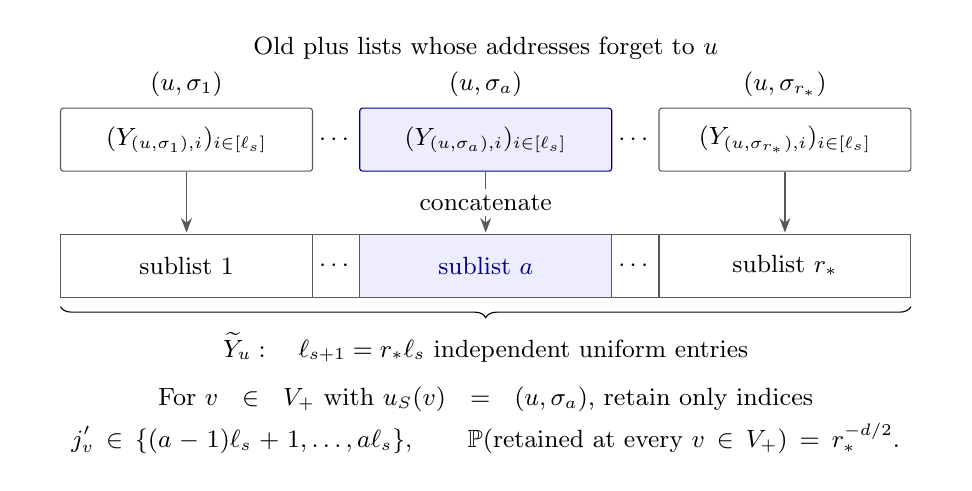
\begin{tikzpicture}[
      x=1cm,y=1cm,>=Stealth,
      every node/.style={font=\small},
      oldlist/.style={draw=black!65,rounded corners=1pt,minimum height=8mm,
        minimum width=32mm,inner sep=2pt},
      guide/.style={draw=black!65,->,line width=.5pt},
      chosen/.style={fill=blue!7,draw=blue!55!black},
      index/.style={text=blue!55!black}
    ]
    \node[anchor=south] at (5.4,.9)
      {Old plus lists whose addresses forget to $u$};
    \node[anchor=south] at (1.6,.42) {$(u,\sigma_1)$};
    \node[anchor=south] at (5.4,.42) {$(u,\sigma_a)$};
    \node[anchor=south] at (9.2,.42) {$(u,\sigma_{r_*})$};
    \node[oldlist] (first) at (1.6,0)
      {$(Y_{(u,\sigma_1),i})_{i\in[\ell_s]}$};
    \node[oldlist,chosen] (middle) at (5.4,0)
      {$(Y_{(u,\sigma_a),i})_{i\in[\ell_s]}$};
    \node[oldlist] (last) at (9.2,0)
      {$(Y_{(u,\sigma_{r_*}),i})_{i\in[\ell_s]}$};
    \node at (3.5,0) {$\cdots$};
    \node at (7.3,0) {$\cdots$};
    \draw[guide] (first.south) -- (1.6,-1.18);
    \draw[guide] (middle.south) -- (5.4,-1.18);
    \draw[guide] (last.south) -- (9.2,-1.18);
    \node[fill=white,inner sep=2pt] at (5.4,-.8) {concatenate};

    \fill[blue!7] (3.8,-1.2) rectangle (7,-2);
    \draw[black!65] (0,-1.2) rectangle (10.8,-2);
    \draw[black!65] (3.2,-1.2) -- (3.2,-2);
    \draw[black!65] (3.8,-1.2) -- (3.8,-2);
    \draw[black!65] (7,-1.2) -- (7,-2);
    \draw[black!65] (7.6,-1.2) -- (7.6,-2);
    \node at (1.6,-1.6) {sublist $1$};
    \node at (3.5,-1.6) {$\cdots$};
    \node[index] at (5.4,-1.6) {sublist $a$};
    \node at (7.3,-1.6) {$\cdots$};
    \node at (9.2,-1.6) {sublist $r_*$};
    \draw[decorate,decoration={brace,mirror,amplitude=4pt}]
      (0,-2.12) -- (10.8,-2.12);
    \node[anchor=north] at (5.4,-2.33)
      {$\widetilde Y_u:\quad \ell_{s+1}=r_*\ell_s\ \text{independent uniform entries}$};

    \node[align=center,text width=11.4cm,anchor=north] at (5.4,-3.02)
      {For $v\in V_+$ with $u_S(v)=(u,\sigma_a)$, retain only indices\\[3pt]
       $\displaystyle j'_v\in\{(a-1)\ell_s+1,\ldots,a\ell_s\},
       \qquad \mathbb P(\text{retained at every }v\in V_+)=r_*^{-d/2}.$};
  \end{tikzpicture}
  \caption{Marking the cut block $b$: the comparison between $S$ and
    $S'=S\cup\{b\}$. For each new address $u$, concatenate its $r_*$ old
    plus lists; the displayed sublists are schematic. Independence and
    probabilities refer to sampling before weights are applied.
    Restricting the new index at each plus slot to its former sublist
    recovers the old distribution of selected labels, with probability
    $r_*^{-d/2}$. Every edge between new addresses
    gives an old edge between every pair of their plus sublists. Hence every
    factor of $I_{S'}$ occurs in $I_+$, and $0\le W\le1$ gives
    $I_{S'}\ge I_+$. These are the two ingredients of the comparison for
    $Q_{S'}(J)$.}
  \label{fig:list-concatenation}
\end{figure}


\subsection{The mixture and its cycle property}

Define a finite measure and its normalization by
\begin{equation}\label{eq:tuple-mixture}
 M=\sum_{\substack{S\subseteq[w]\\|S|\le t+1}}
           p^{-|S|\delta/2}\nu_S,
 \qquad \mu_{l,p}=\frac{M}{M(1)}.
\end{equation}
For a fixed cut in block $b$, pair each $S$ missing $b$, $|S|\le t$,
with $S'=S\cup\{b\}$.  By
\eqref{eq:tuple-unmarked-error} and \eqref{eq:tuple-concatenation}, their
combined quadratic form is at least
\[
 p^{-s\delta/2}
 \bigl(c_*r_*^{-d/2}p^{-\delta/2}-Cp^{-\delta}\bigr)
 \mathcal A_S(J)\ge0
\]
for all sufficiently large $p$.  Every component containing $b$ is
used in exactly one such pair; the remaining components have
$|S|=t+1$, $b\notin S$, and nonnegative quadratic forms.  This proves
reflection positivity of $M$ and hence of $\mu_{l,p}$.

For $S=\varnothing$, every list has length one, all index weights are
one, and the component mass is a graph average.  Therefore
\eqref{eq:tuple-graph-mean} and $c_p\ge1/(2k)$ show that
$\nu_\varnothing(1)\ge c_0>0$ for sufficiently large $p$, uniformly in
$l$.  The uniform upper bounds on all component masses give
\[
 c_0\le M(1)\le C_0.
\]
Define the exceptional submeasure by
\begin{equation}\label{eq:tuple-exceptional}
 \varepsilon_{l,p}
 =\frac{p^{-(t+1)\delta/2}}{M(1)}
       \sum_{|S|=t+1}\nu_S.
\end{equation}
It has mass $O(p^{-(t+1)\delta/2})\le p^{-4}$ after increasing the
prime threshold, by the choice of $t$.

For $|S|\le t$ at least $t+1$ blocks remain unmarked, and the addresses
of $v_j,v_{j+1}$ satisfy \eqref{eq:tuple-address-edge} in every one of
them.  The product $I_S$ therefore includes the weight on every pair of
their list entries.  On its support, in particular, the entries selected
at those two slots have increment in the support of $W$, which consists
of admissible residues.  This proves the cycle property for
$\mu_{l,p}^{\circ}$.  Translating every list entry by the same element
of $\F_p$ leaves all the weights unchanged.  Each component,
and hence both measures in the proposition, is translation invariant.
The assertion about one-slot marginals follows because translation acts
transitively on $\F_p$.

\subsection{Covariance and conditional mixing}

It remains to show that the construction follows the auxiliary family
under affine changes and that conditioning on the other slots reveals
little about a mean-zero function at one slot.  The first property will
permit passage to progressions.  The second will control large
denominators in the Fourier lifts.

If $p\nmid D$, the auxiliary-family identity \eqref{eq:auxiliary-change} gives
\[
 W_{lD,p}(y)=W_{l,p}(\lambda(D)y).
\]
Indeed the substitution $x\mapsto Dx-i$ is bijective modulo $p$,
preserves $T_l(Dx-i)=T_{lD}(x)$, and preserves nonvanishing of the
derivative because both $D$ and $\lambda(D)$ are units modulo $p$.
Consequently changing every list entry to
$\lambda(D)^{-1}(Y_{u,i}-a')$ transforms each component for $l$ into
the component for $lD$, preserving its mass and all index weights.
The mixtures and their exceptional parts therefore satisfy
\eqref{eq:tuple-covariance}.

For \eqref{eq:tuple-mixing}, first consider the normalized component
$\nu_\varnothing/\nu_\varnothing(1)$.  At a fixed slot $v$ write
$x=z_v$ and $y=(z_u)_{u\ne v}$.  Its unnormalized density, relative to
independent uniform labels, factors as
\[
 J_1(x,y)J_2(y),
\]
where $J_1$ is the product of the $m$ edge weights incident with $v$,
and $J_2$ contains the remaining edges.  Put
\[
 A(y)=\mathbb E_xJ_1(x,y),\qquad
 B(y)=\mathbb E_xf(x)J_1(x,y).
\]
Apply \eqref{eq:tuple-graph-operator} to the graph of incident edges,
whose two sides are $\{v\}$ and the other vertices.  Since
$\mathbb E f=0$, it gives
\[
 \|A-c_p^m\|_2\le Cp^{-\delta},\qquad
 \|B\|_2\le Cp^{-\delta}\|f\|_2.
\]
The conditional expectation at $y$ is $B(y)/A(y)$ when $A(y)>0$.
The marginal density of $y$ is
$J_2(y)A(y)/\nu_\varnothing(1)$, so the squared conditional norm is
\begin{equation}\label{eq:tuple-leading-conditional}
 \frac1{\nu_\varnothing(1)}
    \mathbb E_yJ_2(y)\frac{|B(y)|^2}{A(y)},
\end{equation}
with the ratio defined as zero when $A=0$.
On $A\ge c_p^m/2$, this is bounded using the estimate for $B$.
The complementary set has uniform probability $O(p^{-2\delta})$
by the estimate for $A$, since $c_p^m$ is bounded below.  On that set,
weighted Cauchy--Schwarz and $J_1\le1$ give
\[
 \frac{|B(y)|^2}{A(y)}
 \le\mathbb E_x|f(x)|^2J_1(x,y)\le\|f\|_2^2.
\]
Together with $J_2\le1$ and the lower bound on
$\nu_\varnothing(1)$, this proves that
\eqref{eq:tuple-leading-conditional} is
$O(p^{-2\delta})\|f\|_2^2$.

Both $\mu_{l,p}$ and $\mu_{l,p}^{\circ}$ are mixtures of the normalized
components, and in either mixture the total probability of
$S\ne\varnothing$ is $O(p^{-\delta/2})$.  To justify transfer of the
estimate, retain the component label as an additional random variable.
Conditional Jensen shows that conditioning on this label as well as on
all other slots can only increase the squared conditional norm.  In each
normalized component the trivial bound is $\|f\|_2^2$, since that
component has a uniform marginal at slot $v$.  Averaging the leading
estimate and these trivial bounds therefore yields
\[
 \left\|\mathbb E_{\rho_p}
   [f(z_v)\mid(z_u)_{u\ne v}]\right\|_2^2
 \le C p^{-\delta/2}\|f\|_2^2.
\]
As $2\gamma=\delta/5<\delta/2$, increasing the prime threshold makes
this at most $p^{-2\gamma}\|f\|_2^2$.  This proves
\eqref{eq:tuple-mixing} and completes the proof of
Proposition~\ref{prop:tuple-laws}.

Fix henceforth a threshold $P>P_1$ for which the proposition holds, large
enough also that
\begin{equation}\label{eq:prime-thresholds}
 p^{\gamma/2}\ge3\quad(p\ge P),\qquad
 \prod_{p\ge P}(1+p^{-3})-1\le\tfrac14,
\end{equation}
where the product is over primes.  Its tail tends to one because
$\sum_p p^{-3}<\infty$.  Define
\begin{equation}\label{eq:small-prime-modulus}
 M_0=\prod_{p<P}p^{E_p}\ge2.
\end{equation}
The previously chosen $L$ is unchanged when $P$ is enlarged.  For
$D=M_0$ times a product of distinct primes at least $P$, a residue
modulo $D$ is called admissible at $l$ if it is admissible at every local
factor $p^{E_p}$ of $D$.

\section{Multilinear estimates and Fourier lifts}
\label{sec:lifts}

The tuple laws of Section~\ref{sec:tuples} provide two ways to control
multilinear averages: reflection positivity compares different inputs
with a single diagonal quantity, while conditional mixing suppresses
large Fourier denominators.  We develop both estimates, then prove the
moment bounds needed to apply them to bounded functions on integer
intervals.  The signed-form and Fourier-lift arguments follow the corresponding
section of~\cite{IntersectivePower}.  The signed-form estimates have their
square-difference counterpart in~\cite[Proposition~4.1 and
Lemmas~4.2--4.3]{SquarePower}.  We give full proofs of the estimates
needed here.  The
change of coordinates in Lemma~\ref{lem:seminorm} carries the auxiliary
parameter from \(l\) to \(lD\).

Retain the index set \(V=\Pi^w\), where \(\Pi\) consists of the
permutation words on \([L]\), and put \(d=|V|\); in particular, \(d\) is even.
Fix a positive integer
\(l\) and a finite set \(\mathcal P\) of primes at least \(P\).  Set
\[
 X_{\mathcal P}=\prod_{p\in\mathcal P}\F_p,
 \qquad
 \mu_{l,\mathcal P}=\bigotimes_{p\in\mathcal P}\mu_{l,p}.
\]
We collect the prime labels in slot \(v\) into a single variable
\(z_v\in X_{\mathcal P}\), so \(\mu_{l,\mathcal P}\) is a probability
law on \(X_{\mathcal P}^V\).  Each single-slot marginal is uniform.
Norms of functions on \(X_{\mathcal P}\) will always use uniform
probability measure unless another measure is specified.
For real functions on this space define
\[
 \mathcal Z_{l,\mathcal P}((g_v)_{v\in V})
 =\int\prod_{v\in V}g_v(z_v)\,d\mu_{l,\mathcal P},
 \qquad
 Z_{l,\mathcal P}(g)=\mathcal Z_{l,\mathcal P}((g)_{v\in V}).
\]
The empty prime set is allowed: its residue space is a singleton and
\(Z_{l,\varnothing}(g)=g^d\).

We also fix the Fourier notation on these spaces.  Every frequency has a
unique additive decomposition
\[
 \xi=\sum_{p\in\mathcal P}\frac{a_p}{p}\pmod 1,
 \qquad 0\le a_p<p,
\]
and its character is
\(e(z\xi)=\prod_{p\in\mathcal P}e(a_pz_p/p)\).
Equivalently, one may use any integer representative of \(z\) supplied
by the Chinese remainder theorem.  The \emph{exact support} of this
character is \(\{p:a_p\ne0\}\); its reduced denominator, denoted
\(q(\xi)\), is the product of those primes.  For
\(B\subseteq\mathcal P\) write
\(q_B=\prod_{p\in B}p\), with \(q_\varnothing=1\).

\subsection{Signed H\"older inequality and seminorm rules}

The finite reflection argument below follows the chessboard method of
Fr\"ohlich, Israel, Lieb and Simon~\cite[Theorem~4.1]{FILS1978};
related reflection arguments for graph norms appear in Conlon and
Lee~\cite[Section~3]{ConlonLee2017}.
The standard passage from a multilinear H\"older inequality to a seminorm
is also part of Hatami's criterion for graph norms~\cite[Theorem~2.8 of
the arXiv version]{Hatami2010}; we prove both steps directly for the
present tuple laws.

\begin{proposition}[Signed H\"older inequality]
\label{prop:signed-holder}
For every positive integer \(l\), finite set \(\mathcal P\) of primes
at least \(P\), and real functions \(g,g_v:X_{\mathcal P}\to\R\),
\begin{equation}
 Z_{l,\mathcal P}(g)\ge0,
 \qquad
 \left|\mathcal Z_{l,\mathcal P}((g_v)_{v\in V})\right|
 \le\prod_{v\in V} Z_{l,\mathcal P}(g_v)^{1/d}.
 \label{eq:signed-holder}
\end{equation}
\end{proposition}

\begin{proof}
Across any reflection cut of \(V\), the matrix of the product law is
the tensor product of the corresponding prime-law matrices.  It is
therefore positive semidefinite.  To explain its consequence for signed
inputs, fix a cut \(V=V_+\sqcup V_-\) and its reflection \(\theta\).
Define maps \(\phi_\pm:V\to V_\pm\) that fix the selected half and
reflect the other half into it.  An assignment of functions is a map
\(a:v\mapsto g_v\); write its integral as \(\Lambda(a)\).
The two real functions on the plus-half labels that enter the cut
bilinear form are
\[
 F(x)=\prod_{v\in V_+}a(v)(x_v),
 \qquad
 G(x)=\prod_{v\in V_+}a(\theta v)(x_v).
\]
Its mixed value is \(\Lambda(a)\), and its two quadratic values are
\(\Lambda(a\circ\phi_+)\) and \(\Lambda(a\circ\phi_-)\).
Cauchy--Schwarz for the positive semidefinite matrix gives
\begin{equation}
 |\Lambda(a)|^2
 \le \Lambda(a\circ\phi_+)\Lambda(a\circ\phi_-),
 \qquad \Lambda(a\circ\phi_\pm)\ge0.
 \label{eq:fold-cs}
\end{equation}
In particular a constant assignment has nonnegative integral, proving
the first assertion of~\eqref{eq:signed-holder}.

We next give a finite sequence of fold maps that sends every vertex to
one vertex.  In one block write \(p_i\) for the position of symbol
\(i\) in its permutation word.  Folding onto the half where \(i\)
precedes \(i+1\) sorts the pair \((p_i,p_{i+1})\), leaving all other
entries unchanged.  Apply the comparisons \(i=1,\ldots,L-1\) in that
order, and repeat this sweep \(L-1\) times.  A sweep moves the largest
entry to the end.  Once the largest entries occupy their final positions,
the next sweep leaves them there and places the largest remaining entry
immediately before them.  Thus every position array becomes
\((1,\ldots,L)\).  Perform these sweeps in each block.  If their fold
maps in chronological order are \(\phi_1,\ldots,\phi_m\), then
\[
 \phi_m\circ\cdots\circ\phi_1(v)=v_*
 \quad\text{for every }v\in V,
\]
where \(v_*\) has the identity word in every block.

Now fix a finite nonempty list of real functions and let \(M\) be the
maximum absolute integral over all assignments from that list, allowing
repetition.  If \(M>0\), take a maximizing assignment.  Each of its
folded integrals is nonnegative and at most \(M\), while their product
is at least \(M^2\) by~\eqref{eq:fold-cs}.  Both therefore equal
\(M\).  Hence either fold preserves maximality.  Apply the pullbacks
in reverse order, first \(\phi_m\), then \(\phi_{m-1}\), and so on.
The final assignment is
\(a\circ\phi_m\circ\cdots\circ\phi_1\), which is constant.  It
follows that \(M\) is a diagonal value.  Conversely, constant
assignments are included in the maximum.  We have proved that the
maximum absolute mixed integral equals the largest diagonal value in
the list; this is also true when \(M=0\).

For \(\epsilon>0\), apply this conclusion to the list
\[
 \frac{g_v}{(Z_{l,\mathcal P}(g_v)+\epsilon)^{1/d}},
 \qquad v\in V.
\]
Each diagonal value in this list is at most one.  Multilinearity gives
\( |\mathcal Z_{l,\mathcal P}((g_v)_v)|
 \le\prod_v(Z_{l,\mathcal P}(g_v)+\epsilon)^{1/d}\).
Let \(\epsilon\downarrow0\).  This proves the second assertion,
including cases where some diagonal values vanish.
\end{proof}

Define
\[
 \|g\|_{l,\mathcal P}=Z_{l,\mathcal P}(g)^{1/d}
 \quad\text{for real }g.
\]
For \(B\subseteq\mathcal P\), let \(\mathbb E_B g\) mean uniform averaging
over the coordinates in \(B\), with all other coordinates held fixed.
The resulting function may be viewed on either \(X_{\mathcal P}\) or
\(X_{\mathcal P\setminus B}\).

\begin{lemma}[Seminorm and changes of coordinates]
\label{lem:seminorm}
The map \(g\mapsto\|g\|_{l,\mathcal P}\) is a seminorm on the real
functions on \(X_{\mathcal P}\).  It satisfies
\[
 |\mathbb E g|\le\|g\|_{l,\mathcal P},
 \qquad
 \|\mathbb E_Bg\|_{l,\mathcal P\setminus B}
 =\|\mathbb E_Bg\|_{l,\mathcal P}
 \le\|g\|_{l,\mathcal P}.
\]
Translations of the input are isometries.  Moreover, if \(D\) is a
positive integer coprime to every prime of \(\mathcal P\), then for
any \(a'\in X_{\mathcal P}\),
\begin{equation}
 \left\|g\bigl(\lambda(D)^{-1}(\,\cdot-a')\bigr)
       \right\|_{l,\mathcal P}
 =\|g\|_{lD,\mathcal P}.
 \label{eq:lift-transport}
\end{equation}
Here the affine change is interpreted separately at each prime.
\end{lemma}

\begin{proof}
Nonnegativity follows from Proposition~\ref{prop:signed-holder}.
Since \(d\) is even, homogeneity of \(Z\) gives absolute homogeneity
of its \(d\)-th root.  Expanding \(Z(g+h)\) by its slots and applying
\eqref{eq:signed-holder} termwise gives
\[
 Z_{l,\mathcal P}(g+h)
 \le\sum_{S\subseteq V}\|g\|_{l,\mathcal P}^{|S|}
                         \|h\|_{l,\mathcal P}^{d-|S|}
 =\bigl(\|g\|_{l,\mathcal P}+\|h\|_{l,\mathcal P}\bigr)^d.
\]
Taking roots proves the triangle inequality.
Putting \(g\) in one slot and 1 in all others in~\eqref{eq:signed-holder}
proves mean domination, since the single-slot marginal is uniform and
\(Z(1)=1\).

The simultaneous translation invariance of the tuple laws proves that
translations are isometries.  Let \(G_B\subseteq X_{\mathcal P}\)
be the additive subgroup of vectors supported on \(B\).  Then
\[
 (\mathbb E_Bg)(z)=\frac1{|G_B|}\sum_{a\in G_B}g(z+a).
\]
The triangle inequality gives the asserted contraction.  Since
\(\mathbb E_Bg\) is independent of \(B\), the probability laws at those
primes integrate out, proving the equality of the two seminorms.
Finally, \(\lambda(D)\) is a unit at each remaining prime, and
the covariance identity \eqref{eq:tuple-covariance} pushes the product law at \(l\) exactly to that at
\(lD\).  This proves~\eqref{eq:lift-transport}.
\end{proof}

\subsection{Decay at large Fourier denominators}

Conditional mixing gives a different estimate, valid also after
removing the exceptional part of each prime law.  Its proof requires
orthogonality between different exact supports; applying the triangle
inequality to all Fourier coefficients would lose this decay.

\begin{lemma}[Large-denominator estimate]
\label{lem:large-denominator}
Fix \(l\ge1\) and a finite prime set \(\mathcal P\) as above.  At
each prime choose either \(\rho_p=\mu_{l,p}\) or
\(\rho_p=\mu_{l,p}^{\circ}\).  Let \(g_v:X_{\mathcal P}\to\C\)
be arbitrary functions.  If, in one distinguished slot \(v\), every
Fourier coefficient at a denominator at most \(R\) vanishes, where
\(R\ge1\), then
\begin{equation}
 \left|\int\prod_{u\in V}g_u(z_u)\,
                  d\bigotimes_{p\in\mathcal P}\rho_p\right|
 \le R^{-\gamma}\|g_v\|_2
                     \prod_{u\ne v}\|g_u\|_{2(d-1)}.
 \label{eq:large-denominator}
\end{equation}
\end{lemma}

\begin{proof}
At one prime, let \(\mathfrak m_p\) denote the marginal law of the labels in all
slots other than \(v\), and let
\[
 T_p f=\mathbb E_{\rho_p}\bigl(f(z_v)\mid(z_u)_{u\ne v}\bigr).
\]
This is an operator from uniform \(L^2(\F_p)\) to \(L^2(\mathfrak m_p)\).
It preserves constants.  It sends uniform-mean-zero inputs to
\(\mathfrak m_p\)-mean-zero outputs, since \(\mathbb E_{\mathfrak m_p}T_pf=\mathbb E f\).
By the conditional mixing estimate \eqref{eq:tuple-mixing}, its
norm on the mean-zero subspace is at most \(p^{-\gamma}\).

The product law makes the conditional operator for all primes equal
to \(T=\bigotimes_pT_p\): this identity holds first for products of
one-prime functions, by independence across primes, and then for every
function by linearity.  The exact-support \(B\) Fourier space has a
mean-zero factor at primes in \(B\) and a constant factor elsewhere.
On this space the operator norm is at most \(q_B^{-\gamma}\).
Furthermore, the images of two distinct exact-support spaces are
orthogonal in \(L^2(\bigotimes_p\mathfrak m_p)\).  At a prime in the symmetric
difference of the supports, one image factor is constant and the other
has mean zero.  Their inner product is zero, and tensoring preserves
this orthogonality.

Decompose \(g_v=\sum_{q_B>R}g_{v,B}\) by exact supports.  Both the
domain summands and their images are orthogonal, so
\[
 \|Tg_v\|_2^2
 =\sum_{q_B>R}\|Tg_{v,B}\|_2^2
 \le\sum_{q_B>R}q_B^{-2\gamma}\|g_{v,B}\|_2^2
 \le R^{-2\gamma}\|g_v\|_2^2.
\]
Condition the original integral on the other slots and apply
Cauchy--Schwarz.  The remaining factor is bounded by
\[
 \left\|\prod_{u\ne v}g_u(z_u)\right\|_2
 \le\prod_{u\ne v}
       \left(\mathbb E|g_u(z_u)|^{2(d-1)}\right)^{1/(2(d-1))}
 =\prod_{u\ne v}\|g_u\|_{2(d-1)},
\]
using ordinary H\"older and the uniform single-slot marginals.
This proves~\eqref{eq:large-denominator}.  If \(\mathcal P\) is empty, the frequency
hypothesis forces \(g_v=0\), and the conclusion is immediate.
\end{proof}

\subsection{Fourier lifts and uniform moments}

A bounded function on an integer interval gives Fourier coefficients at
rational frequencies.  We transfer a finite set of these coefficients
to \(X_{\mathcal P}\).  Such a transfer need not preserve pointwise
bounds, so we prove bounds for every fixed moment.  The following
proposition and proof reproduce the uniform lift argument
of~\cite[section ``Multilinear estimates and Fourier lifts'']{IntersectivePower}.
For the square-difference setting, see~\cite[Lemmas~5.2--5.3]{SquarePower}.
We must also allow
arbitrary subfamilies of complete exact supports, because fixing some
residue coordinates changes which denominators remain.

Let \(I\) be a nonempty consecutive interval of integers and let
\(f:I\to\C\).  Put
\[
 \widehat f_I(\xi)=\frac1{|I|}\sum_{x\in I}f(x)e(-x\xi).
\]
For \(B\subseteq\mathcal P\), define its exact-support contribution
\[
 f_B(z)=\sum_{q(\xi)=q_B}\widehat f_I(\xi)e(z\xi),
\]
where the frequencies are characters of \(X_{\mathcal P}\).  For
\(Q\ge1\), the Fourier lift is
\[
 \mathcal L_{I,\mathcal P,Q}f(z)
 =\sum_{\substack{B\subseteq\mathcal P\\q_B\le Q}}f_B(z)
 =\sum_{\substack{\xi\text{ on }X_{\mathcal P}\\q(\xi)\le Q}}
                   \widehat f_I(\xi)e(z\xi).
\]
Each \(f_B\) depends only on the coordinates in \(B\), and has mean
zero in each of those coordinates.  If \(f\) is real, all these
functions are real because each summation set is closed under negation.
Retaining a support \(B\) always means retaining all its frequencies.

\begin{proposition}[Uniform lift moments]
\label{prop:lift-moments}
Let \(\mathcal P\) be any finite set of primes, \(Q\ge1\), and let
\(I\) be a consecutive integer interval with \(|I|\ge10Q^6\).
For every integer \(r\ge1\), every \(\epsilon>0\), every function
\(f:I\to\C\), and every subfamily
\(\mathcal F\subseteq\{B\subseteq\mathcal P:q_B\le Q\}\),
\begin{equation}
 \left\|\sum_{B\in\mathcal F}f_B\right\|_{2r}
 \le C_{r,\epsilon}\|f\|_\infty Q^\epsilon.
 \label{eq:lift-moments}
\end{equation}
The constant is independent of the prime set, the interval and its
location, the function, and the subfamily.
\end{proposition}

\begin{proof}
The zero function is immediate; otherwise scale so that
\(\|f\|_\infty\le1\).  Write \(N_I=|I|\), and let
\[
 u=\max\{|B|:B\subseteq\mathcal P,\ q_B\le Q\}.
\]
The empty support is included, so this maximum is defined even when
\(\mathcal P\) is empty.
We first control conditional sums of squares of the \(f_B\), then their
square-function moments.  Symmetrization will recover the moment of
their sum.

\smallskip
\noindent\emph{Conditional energy.}
For \(J\subseteq\mathcal P\) with \(q_J\le Q\), and any fixed
coordinate vector \(z_J\), we claim that
\begin{equation}
 \sum_{\substack{B\in\mathcal F\\B\supseteq J}}
       \mathbb E\bigl(|f_B|^2\mid z_J\bigr)\ll4^{|J|}.
 \label{eq:conditional-energy}
\end{equation}
The conditional expectation here averages uniformly over all coordinates
outside \(J\).  If \(B\supseteq J\), the coefficient of an outside
character \(\eta\) of exact support \(B\setminus J\), after fixing
\(z_J\), is
\[
 c_J(\eta;z_J)
 =\frac1{N_I}\sum_{x\in I}f(x)e(-x\eta)
       \prod_{p\in J}\bigl(p\mathbf 1_{\{x\equiv z_p\pmod p\}}-1\bigr).
\]
Indeed, the sum over the nonzero frequencies at \(p\) is
\(\sum_{a=1}^{p-1}e(a(z_p-x)/p)
=p\mathbf 1_{\{x\equiv z_p\pmod p\}}-1\).
The outside characters associated with \(B\) have exact support
\(B\setminus J\).  These supports distinguish the sets \(B\supseteq J\),
so their character sets are disjoint.  Conditional Parseval therefore
identifies the left side of \eqref{eq:conditional-energy} with the squared
Euclidean norm of this coefficient vector on the union of those sets.

Expand the product in \(c_J\) over subsets \(J'\subseteq J\).
Apart from a sign, the corresponding vector has coordinates
\[
 \frac{q_{J'}}{N_I}
 \sum_{\substack{x\in I\\x\equiv z_{J'}\pmod{q_{J'}}}}
                   f(x)e(-x\eta).
\]
The congruence denotes the class determined by the fixed coordinates in
\(J'\); for the empty subset it imposes no restriction.  Write its
progression as \(x=a+q_{J'}n\), with \(n\) in a consecutive interval
of length \(N'\).  Then
\[
 N'\ge0.9N_I/q_{J'},
 \qquad N'q_{J'}/N_I\le1.1.
\]
In these coordinates the frequencies are \(q_{J'}\eta\), up to
constant phases.  They remain distinct because their denominators are
coprime to \(q_J\).  Their denominators are at most \(Q\), so they
number at most \(Q^2\) and have pairwise circle distance at least
\(Q^{-2}\).

The Gram matrix of these characters in normalized \(L^2\) on the
progression has diagonal 1.  By geometric summation, every off-diagonal
entry has modulus at most \(Q^2/(2N')\).  Its operator norm is
therefore at most its maximum absolute row sum, which is bounded by
\[
 1+\frac{Q^4}{2N'}
 \le1+\frac{Q^5}{1.8N_I}
 \le1+\frac1{18Q}.
\]
To see how this bounds the coefficients, let the synthesis map send
\((b_\eta)_\eta\) to \(\sum_\eta b_\eta e(nq_{J'}\eta)\)
on the progression interval with normalized counting measure.  Its
adjoint is the normalized Fourier analysis map, and its Gram matrix
is the matrix just estimated.  The two maps therefore have norm squared
equal to that Gram-matrix norm.  Since \(\|f\|_\infty\le1\) and
\(N'q_{J'}/N_I\le1.1\), the displayed coefficient vector has
Euclidean norm bounded by an absolute constant.  The triangle inequality
over the \(2^{|J|}\) subsets \(J'\), followed by squaring, proves
\eqref{eq:conditional-energy}.

\smallskip
\noindent\emph{Square-function moments.}
Set
\[
 S(z)=\left(\sum_{B\in\mathcal F}|f_B(z)|^2\right)^{1/2}.
\]
Expand \(\mathbb E S^{2r}\) and fix the supports of its first \(r-1\)
factors.  Their union \(W'\) has size at most \((r-1)u\), and their
product depends only on \(z_{W'}\).  For the final support \(B\),
the function \(f_B\) ignores every coordinate outside \(B\).  Thus
integration outside \(W'\) leaves exactly
\(\mathbb E(|f_B|^2\mid z_J)\), where \(J=B\cap W'\).
Every intersection that occurs satisfies \(q_J\le q_B\le Q\).
For each fixed intersection \(J\), the sum over supports with
\(B\cap W'=J\) is bounded by the larger sum over all \(B\supseteq J\)
in~\eqref{eq:conditional-energy}.  There are at most \(2^{(r-1)u}\) possible
intersections and each has at most \(u\) elements.  Thus
\[
 \mathbb E S^{2r}\le C\,2^{(r-1)u}4^u\mathbb E S^{2r-2}.
\]
The same argument with \(r=1\) uses \(J=W'=\varnothing\).
Iteration gives
\begin{equation}
 \|S\|_{2r}\le C_r^{1+u}.
 \label{eq:lift-square-function}
\end{equation}
The overlaps among supports have now been controlled.  It remains to
bound their sum by this square function with a loss exponential only in
\(u\).

\smallskip
\noindent\emph{Recovering the sum.}
We color the prime coordinates and first retain only terms that use one
coordinate of each color.  This will let us apply a scalar random-sign
estimate one color at a time and use consistent coordinate copies across
the retained terms.  Fix a support size \(j\ge1\) and color every prime coordinate with one
of \(j\) colors.  Call a support \emph{transversal} when it has exactly
one prime of each color, and let \(\mathcal T\) be the transversal
supports in \(\mathcal F\) for this coloring.  Take independent uniform
pairs \(X_p^0,X_p^1\) at every prime.  The operator
\(\operatorname{swap}_p\) interchanges these two copies.  Define
\[
 D_B=\prod_{p\in B}(1-\operatorname{swap}_p)f_B(X^0),
 \qquad B\in\mathcal T.
\]
Averaging over all second copies leaves \(f_B(X^0)\), since every
other term in this expansion has mean zero in at least one copied
coordinate.  Jensen's inequality gives
\[
 \left\|\sum_{B\in\mathcal T}f_B\right\|_{2r}
 \le\left\|\sum_{B\in\mathcal T}D_B\right\|_{L^{2r}(X^0,X^1)}.
\]
Independent swaps preserve the joint law of the copies and multiply
\(D_B\) by the product of the corresponding signs.  Thus for independent
uniform signs \(\epsilon_p\), indexed by primes,
\[
 \left\|\sum_{B\in\mathcal T}D_B\right\|_{L^{2r}(X^0,X^1)}
 =\left\|\sum_{B\in\mathcal T}D_B\prod_{p\in B}\epsilon_p
       \right\|_{L^{2r}(X^0,X^1,\epsilon)}.
\]

For completeness, the scalar sign estimate
\[
 \left\|\sum_i a_i\epsilon_i\right\|_{2r}
 \le C_r\left(\sum_i|a_i|^2\right)^{1/2}
\]
follows by expanding the even moment.  Surviving terms have even
multiplicity at every index.  For nonnegative coefficients their sum is
at most
\[
 \frac{(2r)!}{2^r r!}\left(\sum_i a_i^2\right)^r,
\]
because \((2m)!\ge2^m m!\).  For complex coefficients, take absolute
values of the surviving terms in
\((\sum_i a_i\epsilon_i)^r(\sum_i\overline{a_i}\epsilon_i)^r\)
and use the nonnegative case.  Iterating this estimate over the color
classes gives, for fixed copies,
\[
 \left\|\sum_{B\in\mathcal T}D_B\prod_{p\in B}\epsilon_p
       \right\|_{L^{2r}(\epsilon)}
 \le C_r^j\left(\sum_{B\in\mathcal T}|D_B|^2\right)^{1/2}.
\]
At each step Minkowski is used in the form
\(\| (\sum_i|B_i|^2)^{1/2}\|_{2r}
\le(\sum_i\|B_i\|_{2r}^2)^{1/2}\).
The signs are indexed by individual primes; transversality ensures that
each monomial uses exactly one sign from each color class.

In expanding the swaps in \(D_B\), index its \(2^j\) terms by a choice
of copy for each color.  For any fixed such choice, made consistently
across all supports, the selected prime coordinates have the original
product law.  The triangle inequality in
\(L^{2r}(\ell^2(\mathcal T))\) therefore gives
\[
 \left\|\left(\sum_{B\in\mathcal T}|D_B|^2\right)^{1/2}\right\|_{2r}
 \le2^j\left\|\left(\sum_{B\in\mathcal T}|f_B|^2\right)^{1/2}
       \right\|_{2r}
 \le2^j\|S\|_{2r}.
\]
Consequently the transversal sum has norm at most
\((2C_r)^j\|S\|_{2r}\).

Now average over independent uniform colorings.  A fixed size-\(j\) support is
transversal with probability \(j!/j^j\ge e^{-j}\), where here \(e\)
is Euler's number; the inequality follows from
\(\log(j!)\ge\int_1^j\log x\,dx\).
Thus the full size-\(j\) sum is exactly the coloring average of its
transversal sum divided by this probability.  Minkowski yields
\[
 \left\|\sum_{\substack{B\in\mathcal F\\|B|=j}}f_B\right\|_{2r}
 \le(2eC_r)^j\|S\|_{2r}.
\]
Include the constant term of size zero and sum over \(j\le u\).
Together with~\eqref{eq:lift-square-function}, this bounds the norm of
the full sum by \((C'_r)^{1+u}\).
Finally, the product of \(u\) distinct primes is at least \((u+1)!\),
so \((u+1)!\le Q\).  Hence \(u=o(\log Q)\) as \(Q\to\infty\),
uniformly in the prime set.  For every fixed \(r\) and \(\epsilon>0\),
\((C'_r)^{1+u}\le C_{r,\epsilon}Q^\epsilon\).
Restoring \(\|f\|_\infty\) proves~\eqref{eq:lift-moments} with all the stated
uniformities.
\end{proof}

\begin{lemma}[Specialization of residue coordinates]
\label{lem:lift-specialization}
Let \(B\subseteq\mathcal P\), fix \(z_B\in X_B\), and let
\(G:X_{\mathcal P}\to\C\).  For \(1\le s<\infty\),
\[
 \|G(z_B,\cdot)\|_{L^s(X_{\mathcal P\setminus B})}
 \le q_B^{1/s}\|G\|_{L^s(X_{\mathcal P})}.
\]
In particular, a Fourier lift or a subfamily of its complete supports
satisfies~\eqref{eq:lift-moments} after specialization with the additional factor
\(q_B^{1/(2r)}\).  The same bound holds after retaining either the
remaining denominators at most a given \(H\ge1\), or those greater
than \(H\).
\end{lemma}

\begin{proof}
The specified fiber has uniform probability \(1/q_B\).  Its contribution
to \(\mathbb E|G|^s\) is
\(q_B^{-1}\mathbb E|G(z_B,\cdot)|^s\).  Dropping the other nonnegative
contributions proves the first assertion.  For the last assertion,
a character with original exact support \(C\) retains exact support
\(C\setminus B\) after specialization.  The two cuts therefore arise,
before specialization, from the complete-support subfamilies
\[
 \{C\in\mathcal F:q_{C\setminus B}\le H\},
 \qquad
 \{C\in\mathcal F:q_{C\setminus B}>H\}.
\]
Apply Proposition~\ref{prop:lift-moments} to these subfamilies and then use
the fiber bound.  Combining coefficients can cancel frequencies but
cannot create any outside the indicated ranges.
\end{proof}

In particular, specialize the same set \(B\) of coordinates in every
slot, with possibly different values in different slots.  Applying
\eqref{eq:large-denominator} to the product law on the remaining primes
incurs total specialization factor
\[
 q_B^{1/2}\left(q_B^{1/(2(d-1))}\right)^{d-1}=q_B.
\]
Two specialized \(L^2\) norms incur the same factor.  All moment orders
needed here are fixed after \(h\) is fixed.  Finite products of their
subpower bounds remain subpower; none of these constants depends on
\(l\), the specialized residues, or the retained supports.

\section{Prime estimates}\label{sec:primes}

The kernel construction requires two uniform estimates: an asymptotic
formula for primes in residue classes, and cancellation in polynomial
exponential sums over primes.  We derive the first from a zero-free
half-plane theorem and prove the second by Vaughan's identity and Weyl
differencing.  The latter argument also records why the product cutoff
and the arithmetic coefficients do not obstruct mixed differencing.

For positive integers $n$, put
\[
 \Lambda'(n)=(\log n)\mathbf 1_{\{n\text{ is prime}\}},\qquad
 \Lambda(n)=
 \begin{cases}\log p,&n=p^j\text{ for a prime }p\text{ and }j\ge1,\\
 0,&\text{otherwise}.
 \end{cases}
\]
All sums below run over integers, including sums whose endpoints are
real.  The constants in this section are independent of the lower
coefficients of the polynomial phases.

\subsection{Primes in arithmetic progressions}

Here is the precise analytic input from the companion zero-free theorem.
Only its assertion about Dirichlet $L$-functions is needed.

\begin{theorem}[Zero-free input, {\cite[Theorem~1.1]{ZeroFree}}]
\label{thm:zero-free-input}
For every integer $b\ge1$ and every Dirichlet character $\chi$ modulo
$b$, the Dirichlet $L$-function $L(s,\chi)$ has no zero in
$\Re s>7/8$.  This includes imprimitive characters and the trivial
character of modulus $1$, whose $L$-function is $\zeta(s)$.  A pole at
$s=1$ for a principal character is allowed.
\end{theorem}

\begin{proposition}[Uniform distribution in residue classes]
\label{prop:prime-progressions}
Uniformly for $Y\ge2$, $0\le x\le Y$, integers $b\ge1$, and reduced
residue classes $c$ modulo $b$,
\begin{equation}\label{eq:prime-progression}
 \sum_{\substack{n\le x\\n\equiv c\pmod b}}\Lambda'(n)
 =\frac{x}{\varphi(b)}
   +O\bigl(Y^{31/32}\log^2(2bY)\bigr).
\end{equation}
For a nonreduced class modulo $b>1$, the sum is $O(\log b)$ and has
zero main term.
\end{proposition}

\begin{proof}
Set $\sigma_0=15/16$.  We first prove the logarithmic derivative estimate
\begin{equation}\label{eq:log-derivative}
 \frac{L'}{L}(s,\chi)\ll\log\bigl(2b(2+|\Im s|)\bigr)
\end{equation}
on $\Re s=\sigma_0$, and throughout $\sigma_0\le\Re s\le2$ when
$|\Im s|\ge1$.  The constants are absolute, including for imprimitive
characters.

Write $\delta_\chi=1$ for a principal character and $0$ otherwise, and
let
\[
 G_\chi(s)=(s-1)^{\delta_\chi}L(s,\chi).
\]
Fix radii
$2-\sigma_0<r<R<2-7/8$ and use disks of radius $R$ centered at
$s_t=2+it$.  Theorem~\ref{thm:zero-free-input} makes $G_\chi$
holomorphic and nonvanishing on each disk, with the principal pole
removed.  To bound its size there, use periodicity to write
\[
 \sum_{n\le u}\chi(n)=\overline\chi\,u+E_\chi(u),\qquad
 |E_\chi(u)|\le2b,\qquad
 \overline\chi=\begin{cases}\varphi(b)/b,&\delta_\chi=1,\\0,&\delta_\chi=0.
 \end{cases}
\]
Partial summation continues the Dirichlet series to $\Re s>0$ as
\[
 L(s,\chi)=\overline\chi\,\frac{s}{s-1}
       +s\int_1^\infty E_\chi(u)u^{-s-1}\,du.
\]
Consequently, on the disk,
$|G_\chi(s)|\le C[2b(2+|t|)]^C$.  At its center the absolutely
convergent Euler product gives $|L(2+it,\chi)|\ge\zeta(4)/\zeta(2)$;
hence $|G_\chi(s_t)|$ is bounded below by the same positive constant.
Choose a holomorphic logarithm and subtract its value at $s_t$.
Its real part is bounded above by
$C\log(2b(2+|t|))$.  Borel--Carath\'eodory on an intermediate disk,
followed by Cauchy's estimate on the disk of radius $r$, now gives
\[
 \frac{G_\chi'}{G_\chi}(s)
 \ll\log(2b(2+|t|))\qquad (|s-s_t|\le r).
\]
Subtracting $\delta_\chi/(s-1)$ proves
\eqref{eq:log-derivative} in the asserted ranges.

We next pass through a smoothed sum so that the contour integral is
absolutely convergent.  Mellin inversion for $(1-u)_+$ gives, for $x\ge1$,
\begin{equation}\label{eq:smoothed-character-primes}
 \sum_{n\le x}(x-n)\Lambda(n)\chi(n)
 =\frac{1}{2\pi i}\int_{(2)}
   -\frac{L'}{L}(s,\chi)\frac{x^{s+1}}{s(s+1)}\,ds.
\end{equation}
Here the interchange with the Dirichlet series is absolute.  Move the
line to $\Re s=\sigma_0$.  Estimate~\eqref{eq:log-derivative} bounds
the horizontal integrals by a constant times
$x^3\log(2b(2+T))/T^2$, which tends to zero with the height $T$.
The sole crossed pole is at $s=1$ for the principal character; its
residue is $x^2/2$.  On the new vertical line, integration of
$\log(2b(2+|t|))/(1+t^2)$ gives
\begin{equation}\label{eq:smoothed-character-result}
 \sum_{n\le x}(x-n)\Lambda(n)\chi(n)
 =\delta_\chi\frac{x^2}{2}
      +O\bigl(x^{1+\sigma_0}\log(2b)\bigr).
\end{equation}

For $(c,b)=1$, character orthogonality yields
\[
 A_c(x):=\sum_{\substack{n\le x\\n\equiv c\pmod b}}
                 (x-n)\Lambda(n)
 =\frac{x^2}{2\varphi(b)}
      +O\bigl(x^{1+\sigma_0}\log(2b)\bigr).
\]
There are $\varphi(b)$ character errors and a factor $1/\varphi(b)$,
so the error is uniform in $b$.  Crucially, sharp differencing is now
performed on this nonnegative progression sum, rather than on a complex
character sum.  For $0<H<x$, positivity of $\Lambda$ gives
\[
 \frac{A_c(x)-A_c(x-H)}{H}
 \le \sum_{\substack{n\le x\\n\equiv c\pmod b}}\Lambda(n)
 \le \frac{A_c(x+H)-A_c(x)}{H}.
\]
Take $H=x^{31/32}$ for sufficiently large $x$.  The main terms differ
from $x/\varphi(b)$ by $O(H)$, and the errors are
\[
 O\bigl(x^{1+\sigma_0}/H\cdot\log(2b)\bigr)
   =O\bigl(x^{31/32}\log(2b)\bigr).
\]
Bounded $x$ is harmless.  Finally,
\[
 \sum_{\substack{p^j\le Y\\j\ge2}}\log p
 \ll Y^{1/2}\log^2(2Y),
\]
so removing higher prime powers proves~\eqref{eq:prime-progression}.
If a prime lies in a nonreduced residue class modulo $b$, it divides
$b$; the sum of the logarithms of distinct such primes is at most
$\log b$.  This proves the last assertion.
\end{proof}

\subsection{A minor-arc estimate over primes}

\begin{proposition}[Prime polynomial sums]\label{prop:prime-minor-arcs}
For fixed $k\ge2$ and $0<\rho<1$, there is a constant
$c_m=c_m(k,\rho)\in(0,1/4)$ with the following property.  If $Y$ is
sufficiently large, $I\subseteq[1,Y]$ is an interval, and
$f\in\R[x]$ has degree at most $k$ with coefficient $b_k$ of $x^k$,
then
\begin{equation}\label{eq:prime-minor-arc}
 \left|\sum_{n\in I}\Lambda'(n)e(f(n))\right|
 \ll_{k,\rho}Y^{1-c_m},
\end{equation}
provided $\theta=(k!)^2b_k$ has an approximation $a/q$ satisfying
\begin{equation}\label{eq:minor-rational-range}
 (a,q)=1,\qquad |\theta-a/q|\le q^{-2},\qquad
 Y^\rho\le q\le Y^{k-\rho}.
\end{equation}
\end{proposition}

Vaughan's identity will split the prime weight into sums with one short
variable and bilinear sums.  Weyl differencing turns each into averages
of linear phases, which rational approximation then bounds.  We first
prove the needed spacing and differencing estimates.  Uniformity in the
lower coefficients and in the interval will later permit additive linear
twists for periodic restrictions and partial summation for smooth weights
in the kernel construction.

Write $\|u\|$ for the distance of $u\in\R$ to the
nearest integer, and interpret $\min(M,\|u\|^{-1})$ as $M$ when
$\|u\|=0$.

\begin{lemma}[Rational spacing]\label{lem:rational-spacing}
Suppose $(a,q)=1$, $q\ge2$, and $|\theta-a/q|\le q^{-2}$.
For $R\ge1$ and $M\ge1$,
\begin{equation}\label{eq:rational-spacing}
 \sum_{1\le r\le R}\min(M,\|\theta r\|^{-1})
 \ll (R/q+1)\bigl(M+q\log(2q)\bigr).
\end{equation}
\end{lemma}

\begin{proof}
Within a block of $\lfloor q/2\rfloor$ consecutive integers, two distinct
indices differ by a nonzero $d$ with $|d|<q/2$.  Thus
\[
 \|\theta d\|\ge \|ad/q\|-|d|/q^2\ge1/(2q).
\]
The associated points are $1/(2q)$ separated on the circle.  The nearest
point to zero contributes at most $M$, and summing the others in bands
of width $1/(2q)$ gives $O(q\log(2q))$, with another $O(M)$ for the
bounded number of points in the first band.  Partitioning the indices
into such blocks proves the result, also when $q=2$ or $3$.
\end{proof}

We will repeatedly group a fixed number of nonzero integer factors by
their product.  If that product has absolute value at most $Y^{C_k}$,
the number of such factorizations is $Y^{o(1)}$, uniformly in the
product.  Indeed, its prime factorization bounds the number by a fixed
order divisor function, up to a bounded number of sign choices.  For
every $\epsilon>0$ that function is $O_{k,\epsilon}(Y^\epsilon)$:
allocating a prime exponent among finitely many factors gives a
polynomial in the exponent, which is bounded by any fixed positive
power of the prime power after allowing a constant for finitely many
small primes.

The following two differencing bounds isolate the treatment of
coefficients and summation domains.  They are forms of classical Weyl
differencing; see \cite{Weyl1916,Vaughan1997} for the method.

\begin{lemma}[One-variable and mixed differencing]
\label{lem:prime-differencing}
Let $k\ge2$, and let $f\in\R[x]$ have degree at most $k$, with
coefficient $b_k$ of $x^k$.

If $J$ is an interval of integers of length at most an integer $M\ge1$,
and $m$ is a positive integer, then
\begin{equation}\label{eq:type-one-differencing}
 \left|\frac1M\sum_{n\in J}e(f(mn))\right|^{2^{k-1}}
 \ll_k\frac1{M^k}
 \sum_{|u_1|,\ldots,|u_{k-1}|<M}
 \min\bigl(M,\|k!b_km^ku_1\cdots u_{k-1}\|^{-1}\bigr).
\end{equation}

Next let $A,B$ be positive integers, let $I\subseteq[1,Y]$ be an
interval, and let $|a_m|,|d_n|\le1$.  Set
\[
 S=\sum_{\substack{A\le m<2A\\B\le n<2B}}
       a_md_n\mathbf 1_{\{mn\in I\}}e(f(mn)),\qquad
 \theta=(k!)^2b_k.
\]
Then
\begin{equation}\label{eq:type-two-differencing}
 \left|\frac{S}{AB}\right|^{2^{2k-1}}
 \ll_k\frac1{A^kB^k}
 \sum_{\substack{|u_1|,\ldots,|u_k|<B\\
                  |v_1|,\ldots,|v_{k-1}|<A}}
 \min\bigl(A,\|\theta u_1\cdots u_kv_1\cdots v_{k-1}\|^{-1}\bigr).
\end{equation}
Zero shifts are included in both sums.
\end{lemma}

\begin{proof}
We give the mixed argument explicitly.  For a function $g$ of two
integer variables, define
\[
 \Delta^n_u g(m,n)=g(m,n+u)-g(m,n),\qquad
 \Delta^m_v g(m,n)=g(m+v,n)-g(m,n).
\]
Let $D_0$ be the set of pairs in the displayed box with $mn\in I$.
Extend $a_m$ and $d_n$ by zero outside their respective intervals,
and extend every summand by zero outside $D_0$.  Cauchy--Schwarz first
removes $a_m$:
\[
 \left|\frac{S}{AB}\right|^2
 \le\frac1A\sum_{A\le m<2A}
       \left|\frac1B\sum_n d_n\mathbf 1_{D_0}(m,n)e(f(mn))\right|^2.
\]
Expanding the square and grouping by $u=n'-n$ bounds its right side by
\[
 \frac1B\sum_{|u|<B}
 \left|\frac1{AB}\sum_{m,n}
    d_{n+u}\overline{d_n}\,
    \mathbf 1_{D_0}(m,n+u)\mathbf 1_{D_0}(m,n)
    e\bigl(\Delta^n_u f(mn)\bigr)\right|.
\]
For fixed $u$ the new weight depends only on $n$ and has modulus at
most one.  This is exactly the form needed for another $n$-difference.
In particular, the product cutoff remains inside the sum; it has not
been replaced by a rectangular domain.

For $j$ fixed shifts $\mathbf u=(u_1,\ldots,u_j)$, let
\[
 \begin{split}
 D_{\mathbf u}&=\{(m,n):
      (m,n+\varepsilon\cdot\mathbf u)\in D_0
                   \text{ for every }\varepsilon\in\{0,1\}^j\},\\
 F_{\mathbf u}(m,n)&=
    \Delta^n_{u_j}\cdots\Delta^n_{u_1}f(mn).
 \end{split}
\]
The accompanying coefficient $d_{\mathbf u}(n)$ is defined recursively
by $d_\varnothing(n)=d_n$ and
\[
 d_{(\mathbf u,u)}(n)
   =d_{\mathbf u}(n+u)\overline{d_{\mathbf u}(n)}.
\]
It depends only on $n$ and is bounded by one.  At each subsequent step,
Cauchy--Schwarz in the existing shifts costs only a constant depending
on $j$, because their total normalized mass is at most $2^j$.
Cauchy--Schwarz in $m$, followed by the same square expansion, adds one
$n$-shift.  Induction therefore gives
\begin{equation}\label{eq:n-difference-stage}
 \left|\frac{S}{AB}\right|^{2^k}
 \ll_k\frac1{B^k}\sum_{|u_1|,\ldots,|u_k|<B}
 \left|\frac1{AB}\sum_{m,n}
       d_{\mathbf u}(n)\mathbf 1_{D_{\mathbf u}}(m,n)
       e(F_{\mathbf u}(m,n))\right|.
\end{equation}
All summands still have $m$ and $n$ in their original intervals, as the
zero vertex of every translated cube belongs to $D_0$.

After $k$ differences in $n$, every lower-degree term vanishes, and
\[
 F_{\mathbf u}(m,n)=k!b_k u_1\cdots u_k m^k.
\]
For $0\le j\le k-1$ and $m$-shifts
$\mathbf v=(v_1,\ldots,v_j)$, define the domains
\[
 \begin{split}
 D_{\mathbf u,\mathbf v}=\{(m,n):\;&
 (m+\eta\cdot\mathbf v,n+\varepsilon\cdot\mathbf u)\in D_0\\
 &\text{for every }\eta\in\{0,1\}^j,
                         \ \varepsilon\in\{0,1\}^k\}.
 \end{split}
\]
Thus $D_{\mathbf u,\varnothing}=D_{\mathbf u}$.  For $1\le j\le k-1$, let
\[
 T_{\mathbf u,\mathbf v}
 =\frac1{AB}\sum_{m,n}\mathbf 1_{D_{\mathbf u,\mathbf v}}(m,n)
 e\bigl(\Delta^m_{v_j}\cdots\Delta^m_{v_1}F_{\mathbf u}(m,n)\bigr).
\]
To enter this unweighted family, remove $d_{\mathbf u}$ by
Cauchy--Schwarz in $n$:
\[
 \left|\frac1{AB}\sum_{m,n}
 d_{\mathbf u}(n)\mathbf 1_{D_{\mathbf u}}(m,n)e(F_{\mathbf u}(m,n))
 \right|^2
 \le\frac1B\sum_{B\le n<2B}
 \left|\frac1A\sum_m
    \mathbf 1_{D_{\mathbf u}}(m,n)e(F_{\mathbf u}(m,n))\right|^2.
\]
Expanding the square bounds this by
$A^{-1}\sum_{|v_1|<A}|T_{\mathbf u,(v_1)}|$.
This is the first $m$-differencing step, so removing the coefficients
requires no additional squaring.  For $1\le j\le k-2$, Cauchy--Schwarz
in $n$ and the same square expansion give
\[
 |T_{\mathbf u,\mathbf v}|^2
 \le\frac1A\sum_{|v|<A}|T_{\mathbf u,(\mathbf v,v)}|.
\]
Applying Cauchy--Schwarz also to all existing shift variables, whose
total normalized mass is bounded in terms of $k$, now yields
\begin{equation}\label{eq:m-difference-stage}
 \left|\frac{S}{AB}\right|^{2^{k+j}}
 \ll_k\frac1{B^kA^j}
 \sum_{\substack{|u_1|,\ldots,|u_k|<B\\|v_1|,\ldots,|v_j|<A}}
          |T_{\mathbf u,\mathbf v}|\qquad(1\le j\le k-1).
\end{equation}
This accounts for all $k+(k-1)$ squarings.

Take $j=k-1$.  For fixed $n$, the section of $D_{\mathbf u,\mathbf v}$
is an interval of $m$'s, possibly empty.  In fact each
condition puts $m+\eta\cdot\mathbf v$ in $[A,2A)$ and its product with
the positive number $n+\varepsilon\cdot\mathbf u$ in $I$; it therefore
specifies an interval in $m$.  Their intersection is an interval of
length at most $A$.  The final phase
$\Delta^m_{v_{k-1}}\cdots\Delta^m_{v_1}F_{\mathbf u}$ is linear in $m$
with coefficient
\[
 (k!)^2b_k\,u_1\cdots u_kv_1\cdots v_{k-1}.
\]
A geometric-sum estimate bounds each $m$-sum by the corresponding
minimum in~\eqref{eq:type-two-differencing}.  Summing over at most $B$
values of $n$, the remaining normalized sum is bounded by that minimum
divided by $A$.  The shifts have normalizing factor
$B^{-k}A^{-(k-1)}$, which proves~\eqref{eq:type-two-differencing}.

For~\eqref{eq:type-one-differencing}, perform the same square expansion
$k-1$ times in a single variable.  The translated intersections of $J$
are intervals of length at most $M$, and the final linear coefficient
is $k!b_km^ku_1\cdots u_{k-1}$.  The normalizing factor is
$M^{-(k-1)}$, followed by $M^{-1}$ for the final geometric sum.
This proves the first bound as well.
\end{proof}

\begin{proof}[Proof of Proposition~\ref{prop:prime-minor-arcs}]
We now apply the differencing bounds to Vaughan's decomposition.
We first prove the estimate with $\Lambda$ in place of $\Lambda'$.
Put $e_0=\rho/(100k)$ and $Z=Y^{e_0}$.  For an arithmetic function
$g$, write $g_{\le Z}(n)=g(n)\mathbf 1_{\{n\le Z\}}$ and
$g_{>Z}=g-g_{\le Z}$.  Let $\mu$ denote the M\"obius function, let
$1$ denote the constant arithmetic function, and use $*$ for Dirichlet
convolution.  Vaughan's identity, in the form used here, is
\begin{equation}\label{eq:vaughan-identity}
 \Lambda=\Lambda_{\le Z}+\mu_{\le Z}*\log
       -\mu_{\le Z}*\Lambda_{\le Z}*1
       +\mu_{>Z}*1*\Lambda_{>Z}.
\end{equation}
This decomposition is classical; see \cite[Chapter~3]{Vaughan1997}.
It follows directly from $\log=1*\Lambda$ and
$\mu*1=\mathbf 1_{\{1\}}$: split $\mu$ at $Z$ in $\mu*\log$, and then
split $\Lambda$ at $Z$ in the term $\mu_{>Z}*1*\Lambda$.

\emph{The two sums with a short variable.}
The middle two terms of~\eqref{eq:vaughan-identity} reduce to sums
with an outer variable $m\le Z^2$ and an inner variable $n\le Y/m$.
The outer coefficient is either $\mu(m)$ or
$\sum_{ab=m,\,a,b\le Z}\mu(a)\Lambda(b)$, and therefore has size
$Y^{o(1)}$.  The inner weight is respectively $\log n$ or $1$.
Fix $m$, let $M=\lceil Y/m\rceil$, and consider any interval subsum
$S_m=\sum_{n\in J}e(f(mn))$ of the inner sum.

Apply~\eqref{eq:type-one-differencing}.  For every integer $r$,
\[
 \min(M,\|k!b_kr\|^{-1})
 \le k!\min(M,\|\theta r\|^{-1}),
\]
since $\|k!u\|\le k!\|u\|$.  Tuples with a zero shift contribute
$O_k(M^{-1})$ after normalization.  For the others group by
$r=m^k|u_1\cdots u_{k-1}|\le m^kM^{k-1}$ and apply
Lemma~\ref{lem:rational-spacing}.  The divisor bound gives
\begin{equation}\label{eq:type-one-saving}
 \left|\frac{S_m}{M}\right|^{2^{k-1}}
 \ll Y^{o(1)}\left(
 \frac1M+\frac{m^k}{q}+\frac{m^k}{M}
       +\frac1{M^{k-1}}+\frac q{M^k}\right).
\end{equation}
Here and below logarithmic factors are included in $Y^{o(1)}$.
For completeness, the four terms after $1/M$ result from expanding
\[
 M^{-k}\left(\frac{m^kM^{k-1}}q+1\right)(M+q\log(2q)).
\]
As $m\le Y^{2e_0}$ and $M\ge Y^{1-2e_0}$,
\[
 \frac{m^k}{q},\ \frac q{M^k}\le Y^{-\rho+2ke_0},\qquad
 \frac{m^k}{M}\le Y^{-1+2(k+1)e_0}.
\]
The remaining terms also save a positive power of $Y$.  Taking the
$2^{k-1}$-st root in~\eqref{eq:type-one-saving} therefore gives
$S_m\ll M Y^{-c}$ for some $c=c(k,\rho)>0$, uniformly in the subinterval.
Partial summation permits the weight $\log n$ with a further
$O(\log Y)$ factor.  Since
\[
 \sum_{m\le Z^2}\lceil Y/m\rceil\ll Y\log(2Y),
\]
both short-variable terms save a fixed power of $Y$ after including
the outer coefficients.

\emph{The bilinear sum.}
For the final term of~\eqref{eq:vaughan-identity}, group the factors as
$(\mu_{>Z}*1)(m)\Lambda_{>Z}(n)$.  Each coefficient is $Y^{o(1)}$
when $mn\le Y$, and a nonzero coefficient requires both $m>Z$ and
$n>Z$.  Partition into dyadic boxes
\[
 A\le m<2A,\qquad B\le n<2B,
 \qquad A,B\ge Z/2,\qquad AB\le Y.
\]
There are $O(\log^2(2Y))$ relevant boxes.  Divide out the coefficient
bounds to reduce to $|a_m|,|d_n|\le1$.  If $AB<Y^{1-e_0}$,
the trivial estimate is already sufficient.  Otherwise put
$R=A^{k-1}B^k$ and apply~\eqref{eq:type-two-differencing}.

There are $k$ shifts of range $B$ and $k-1$ of range $A$.
Tuples containing a zero shift contribute
$O_k(A^{-1}+B^{-1})$.  Group the others by their nonzero absolute
product, at most $R$.  Lemma~\ref{lem:rational-spacing} and the divisor
bound imply
\begin{equation}\label{eq:type-two-saving}
 \left|\frac{S}{AB}\right|^{2^{2k-1}}
 \ll Y^{o(1)}\left(
 \frac1A+\frac1B+\frac1q+\frac1R+\frac q{AR}\right).
\end{equation}
Indeed the nonzero-shift bound before expansion is
\[
 \frac{Y^{o(1)}}{AR}(R/q+1)(A+q\log(2q));
\]
the additional term $O(\log(2q)/A)$ is included in $Y^{o(1)}/A$.
Now $A,B\ge Y^{e_0}/2$, while
\[
 AR=(AB)^k\ge Y^{k(1-e_0)},\qquad
 \frac q{AR}\le Y^{-\rho+ke_0}.
\]
Thus~\eqref{eq:type-two-saving} saves a fixed power.  Restoring the
coefficients and summing the boxes preserves a positive saving.

The remaining term $\Lambda_{\le Z}$ costs only $O(Z\log(2Z))$.
This proves the required estimate for $\Lambda$, with some positive
exponent depending only on $k,\rho$.  Removing higher prime powers
costs $O(Y^{1/2}\log^2(2Y))$, as in
Proposition~\ref{prop:prime-progressions}.  Decreasing the exponent
if necessary gives $c_m\in(0,1/4)$ and proves
\eqref{eq:prime-minor-arc}.
\end{proof}

\section{A kernel on differences at prime arguments}\label{sec:kernel}

The tuple laws prescribe a distribution of admissible increments along each
edge of the distinguished cycle.  We now realize its low-denominator Fourier
multipliers by a signed kernel supported on polynomial values at prime
arguments.  This will turn avoidance of those values into cancellation for a
pair of Fourier lifts.  The kernel comparison adapts the integer-argument
method of \cite{IntersectivePower}; the unit conditions in its local weights
and their realization using prime arguments are the additional ingredients
here.

\subsection{Parameters and the pair estimate}

Fix the following parameters, all depending only on $h$ and the tuple
construction:
\begin{equation}\label{eq:parameters}
\begin{split}
 &\eta=\frac{1}{10000k},\qquad
 c_m=c_m(k,\eta/4)\quad\text{from Proposition~\ref{prop:prime-minor-arcs}},
 \qquad \nu=\frac{\min(\eta,c_m/k)}{10},\\
 &\beta=\frac{\nu}{100},\qquad \zeta=\frac{\nu}{100},\qquad
 \tau=\frac{\beta\gamma}{1000k(d+1)},\qquad
 \sigma=\frac{\gamma\tau}{4}.
\end{split}
\end{equation}
Here $\eta$ controls the major arcs, $\nu$ is a common saving from prime
sums, $\beta$ controls the Fourier cutoffs, and $\zeta$ bounds the
auxiliary parameter $l$.  The smaller exponents $\tau$ and $\sigma$ are
reserved for the descent in Section~\ref{sec:descent}.
The parameter $\eta$ is distinct from the exceptional masses $\eta_{l,p}$.
For a scale $N$ put
\begin{equation}\label{eq:kernel-cutoffs}
 Q=N^\beta,\qquad H=N^{\beta/2},\qquad
 \mathcal P_N=\{p\text{ prime}:P\le p\le Q\}.
\end{equation}

Fix $l\ge1$, write $F=h_l$, and choose a directed cycle edge
$v_j\to v_{j+1}$.  For each $p\ge P$, let $\pi_p$ be the distribution on
$\F_p$ of $z_{v_{j+1}}-z_{v_j}$ under $\mu_{l,p}^\circ$.  It is
supported on admissible residues by Proposition~\ref{prop:tuple-laws}.
For $v\in\Z$ define
\[
 \Gamma_p(v/p)=\sum_{y\in\F_p}\pi_p(y)e(vy/p).
\]
For a nonzero character, the conditional mixing estimate
\eqref{eq:tuple-mixing}, applied to the second endpoint and paired with the
conjugate character at the first, gives $|\Gamma_p(v/p)|\le p^{-\gamma}$.
If $\xi$ has squarefree denominator supported on primes at least $P$, write
$\xi=\sum_{p\mid q(\xi)}\xi_p$ for its prime-denominator decomposition and
put $\Gamma(\xi)=\prod_{p\mid q(\xi)}\Gamma_p(\xi_p)$.  Thus
\begin{equation}\label{eq:edge-multiplier-bound}
 \Gamma(0)=1,\qquad |\Gamma(\xi)|\le q(\xi)^{-\gamma}.
\end{equation}
The multiplier may depend on $l$ and the chosen edge; all estimates below
are uniform in both.

\begin{proposition}[Cancellation for an ordered pair]\label{prop:pair-cancellation}
Suppose $N$ is sufficiently large, $l\le N^\zeta$, and
$D=M_0\prod_{p\in B}p\le N^\beta$, where $B$ is a finite set of primes at
least $P$.  Let $J_1,J_2:[N]\to\C$ have modulus at most one and be
supported on residue classes $a'_1,a'_2\pmod D$.  Assume that
$r=a'_2-a'_1\pmod D$ is admissible at $l$ and that
\[
 J_1(x)J_2(y)\ne0\quad\Longrightarrow\quad
 x<y\quad\text{and}\quad y-x\notin\mathcal D_l.
\]
Set
\[
 \Xi=\{\xi\in\Q/\Z:q(\xi)\le H,
       \ q(\xi)\text{ squarefree},\ (q(\xi),D)=1\}.
\]
Then, for the multiplier of any directed cycle edge,
\begin{equation}\label{eq:pair-cancellation}
 D\left|\sum_{\xi\in\Xi}\Gamma(\xi)
       \widehat{J_1}_{[N]}(-\xi)\widehat{J_2}_{[N]}(\xi)\right|
 \ll H^{-\gamma/2}.
\end{equation}
\end{proposition}

Since $M_0$ contains every prime below $P$, the multiplier is defined on all
of $\Xi$.  To prove the proposition, consider the model kernel
\begin{equation}\label{eq:model-kernel}
 k_0(n)=\frac DN\,
   \mathbf1_{\{1\le n\le N\}}\mathbf1_{\{n\equiv r\ (D)\}}
   \sum_{\xi\in\Xi}\Gamma(\xi)e(-\xi n).
\end{equation}
We will construct a kernel $k_1$ supported on $\mathcal D_l$ such that
$\sup_\alpha|\sum_n(k_0(n)-k_1(n))e(\alpha n)|\ll H^{-\gamma/2}$.
The congruence restriction
in $k_0$ will be imposed on polynomial arguments by a local weight; the
factors $\Gamma_p$ will be imposed by further weights of mean one.

\subsection{Weights on polynomial arguments}

For a periodic function of the argument $m$, its \emph{unit mean modulo
$b$} is the uniform average over the classes $m\pmod b$ satisfying
$(T_l(m),b)=1$.  There are exactly
\begin{equation}\label{eq:unit-mean-count}
 n_b=b\prod_{\substack{p\mid b\\p\nmid l}}(1-1/p)
     =\frac{\varphi(lb)}{\varphi(l)}
\end{equation}
such classes.  Indeed, a prime dividing $l$ excludes no argument because
$(r_l,l)=1$, and any other prime excludes exactly one class modulo that
prime.  These means factor over prime powers.  They are also consistent
under replacing $b$ by a multiple: each allowed class has the same number
of allowed lifts.

At a prime $p\mid D$, choose an argument witnessing admissibility of
$r\pmod {p^{E_p}}$, and denote the valuation of its derivative by $s_p$.
Lemma~\ref{lem:local-lifting} supplies a class modulo $p^{E_p-s_p}$ on
which the unit condition holds and $F$ is constantly $r$ modulo
$p^{E_p}$.  Uniform argument lifts in this class give uniform higher
lifts of that value.  Combining the chosen classes gives one class modulo
\[
 d_r=\prod_{p\mid D}p^{E_p-s_p}\mid D.
\]
Let $\rho_D$ be $n_{d_r}$ times its indicator.  Then $\rho_D$ has unit mean
one and $\|\rho_D\|_\infty\le D$.

For every prime $p\nmid D$, necessarily $p\ge P$, choose, for each $y$
with $\pi_p(y)>0$, one allowed regular argument $x_y\pmod p$ satisfying
$F(x_y)=y$.  Define a function $\psi_p$ modulo $p$ by
\[
 \psi_p(x_y)=n_p\pi_p(y),\qquad
 \psi_p(x)=0\quad\text{at all other classes}.
\]
It has unit mean one, and its weighted $F$-value distribution is precisely
$\pi_p$.  Put
\[
 B_p(m)=\psi_p(m)-1,\qquad
 B_u(m)=\prod_{p\mid u}B_p(m),\qquad B_1=1,
\]
where $u$ is squarefree and $(u,D)=1$.  Each $B_p$ has unit mean zero,
$B_u$ has period $u$, and $|B_u|\le u$.  In particular these definitions
specify the weights also on nonunit arguments; those arguments will have
zero main term in the prime-progression estimate.

Expanding a finite product of $\psi_p=1+B_p$ produces a sum of the $B_u$
over squarefree products of those primes.  We retain $u\le H$ to bound
the periods of the weights.  In a unit average against a rational phase
$e(\alpha F(m))$, any prime factor of $u$ absent from $q(\alpha)$ makes
that term vanish.  Thus, when the part of $q(\alpha)$ supported away from
$D$ is at most $H$, the truncation retains every potentially nonzero term
of the corresponding product expansion.  The comparison below will also
bound the contribution from larger denominators.

By Lemma~\ref{lem:auxiliary}, all coefficients of $F$ are $O_h(a_l)$.
Consequently there is an integer $x_*\ge1$, independent of $l$, such that
for $x\ge x_*$,
\begin{equation}\label{eq:kernel-polynomial-scale}
 F(x)\asymp a_lx^k,\qquad F'(x)\asymp a_lx^{k-1},\qquad
 |F''(x)|\ll a_lx^{k-2},
\end{equation}
with $F,F'$ positive.  Put $U=(N/a_l)^{1/k}$.  Since $a_l$ is a positive
integer and $a_l\le al^k$,
\[
 U\le N^{1/k},\qquad U\gg N^{1/k-\zeta}.
\]
For large $N$ there is therefore a unique $X\ge x_*$ with $F(X)=N$, and
$X\asymp U$.  With $\Lambda'(n)=(\log n)\mathbf1_{\{n\text{ prime}\}}$,
define the signed kernel below.  The factor $\varphi(l)/l$ compensates
for the prime density in the progression $T_l(m)$, and $F'(m)/N$ turns
the resulting $m$-integral into normalized measure on the $F$-values:
\begin{equation}\label{eq:prime-kernel}
\begin{split}
 k_1(n)=\sum_{x_*<m\le X}&\mathbf1_{\{n=F(m)\}}
 \frac{F'(m)}{N}\frac{\varphi(l)}{l}\Lambda'(T_l(m))\rho_D(m)\\[-2pt]
 &\hspace{15mm}\times
 \sum_{\substack{u\le H\\u\text{ squarefree}\\(u,D)=1}}B_u(m).
\end{split}
\end{equation}
Here and below the argument $m$ is an integer in sums.  Every nonzero
term has $0<F(m)\le N$ and $T_l(m)$ prime, so $k_1$ is supported on
$\mathcal D_l\cap[N]$.  No positivity is required of $k_1$.

Choose a fixed constant $C$ so that $Y=ClU$ bounds $T_l(X)$.  The relation
$a_l=al^k/\lambda(l)$ gives
\begin{equation}\label{eq:prime-kernel-range}
 Y\gg N^{1/k},\qquad Y\ll N^{1/k+\zeta},\qquad
 Y^k\asymp N\lambda(l).
\end{equation}
In particular $Y\le N$ for sufficiently large $N$.

\subsection{Uniform Fourier comparison}

For $i=0,1$ use positive-sign transforms
$S_i(\alpha)=\sum_n k_i(n)e(\alpha n)$ on $\R/\Z$.
The signs differ from the negative-sign convention for Fourier
coefficients of functions; this choice makes $S_0$ concentrate at the
frequencies occurring in \eqref{eq:model-kernel}.

\begin{lemma}[Comparison of the two kernels]\label{lem:kernel-comparison}
For the data and ranges of Proposition~\ref{prop:pair-cancellation},
\begin{equation}\label{eq:kernel-comparison}
 \sup_{\alpha\in\R/\Z}|S_0(\alpha)-S_1(\alpha)|
 \ll H^{-\gamma/2}.
\end{equation}
\end{lemma}

\begin{proof}
Use major arcs of radius $3N^{-1+\eta}$ around the reduced rationals with
denominator at most $N^\eta$.  They are disjoint for large $N$, since
$3\eta<1$.  The remaining points form the minor arcs.  We first bound both
transforms on the minor arcs; on a major arc we will compare their local
coefficients.

Write $V_N(y)=N^{-1}\sum_{n\in[N]}e(yn)$.  Expanding the congruence
indicator in \eqref{eq:model-kernel} gives
\begin{equation}\label{eq:model-transform}
 S_0(\alpha)=\sum_{\xi\in\Xi}\sum_{j'\bmod D}
 \Gamma(\xi)e(-j'r/D)V_N(\alpha-\xi+j'/D).
\end{equation}
There are $O(DH^2)$ terms.  Their centers $\xi-j'/D$ are distinct:
an equality would give a rational with denominator both coprime to $D$
and dividing $D$, and hence an integer.  Each center has denominator at
most $DH\le N^{3\beta/2}\le N^\eta$.  On minor arcs, geometric summation
therefore gives
\begin{equation}\label{eq:model-minor}
 |S_0(\alpha)|\ll DH^2N^{-\eta}.
\end{equation}

To estimate $S_1$, first consider, with any linear twist $y'$, the sums
\[
 \sum_{m\in I}\Lambda'(T_l(m))e(\alpha F(m)+y'm)
\]
over subintervals $I$ of $(x_*,X]$.  On setting $n=T_l(m)$, expand the
restriction $n\equiv r_l\pmod l$ as the average of its $l$ additive
characters.  Each resulting prime sum has a polynomial phase in $n$ whose
coefficient of $n^k$ is $b_k=\alpha a/\lambda(l)$; the new twists change
only the linear coefficient because $k\ge2$.

Fix a representative of $\alpha$ and apply Dirichlet approximation to
$\vartheta=(k!)^2b_k$ with
\[
 Q_0=\lfloor Y^kN^{-\eta/2}\rfloor.
\]
The resulting reduced fraction $a'/q$ satisfies
$q\le Q_0$ and $|\vartheta-a'/q|\le1/(qQ_0)\le q^{-2}$.
By \eqref{eq:prime-kernel-range}, this places $\alpha$ within
$O(N^{-1+\eta/2})$ of a rational of denominator at most $(k!)^2aq$.
For a minor-arc point that denominator must exceed $N^\eta$ for large
$N$.  Hence, using $Y\le N$ and absorbing the fixed factor $(k!)^2a$,
\[
 Y^{\eta/4}\le q\le Y^{k-\eta/4}.
\]
Proposition~\ref{prop:prime-minor-arcs} applies uniformly in the linear
twists and in the interval, and gives a bound $O(Y^{1-c_m})$.
The relation $Y=ClU$ and the lower bound in
\eqref{eq:prime-kernel-range} imply
\[
 Y^{1-c_m}\ll U\,lN^{-c_m/k}
 \le U N^{\zeta-c_m/k}\ll U N^{-\nu}.
\]
This accounts for the dependence on $l$ before any periodic weight is
expanded.

By \eqref{eq:kernel-polynomial-scale}, the supremum and total variation of
$F'/N$ on $[x_*,X]$ are $O(U^{-1})$.  Partial summation therefore retains
an $O(N^{-\nu})$ bound after including this weight.  Use normalized
Fourier coefficients on each finite period for the other weights.  Since
$\rho_D$ is a constant times one residue-class indicator, its Fourier
$\ell^1$ norm is $n_{d_r}\le D$.  For $B_u$ the bound by its period times
its supremum gives Fourier $\ell^1$ norm at most $u^2$.  Expanding the
weights in \eqref{eq:prime-kernel}, and using $\varphi(l)/l\le1$, yields
\begin{equation}\label{eq:prime-minor-kernel}
 |S_1(\alpha)|\ll D\sum_{u\le H}u^2N^{-\nu}
 \ll DH^3N^{-\nu}.
\end{equation}
The powers in \eqref{eq:model-minor} and
\eqref{eq:prime-minor-kernel} are $2\beta-\eta$ and
$5\beta/2-\nu$, respectively.  Both are smaller than $-\beta\gamma/4$,
so these bounds are $O(H^{-\gamma/2})$.

Now let $\alpha=\alpha_0+y$ be on a major arc, with
$q=q(\alpha_0)\le N^\eta$ and $|y|\le3N^{-1+\eta}$.
Decompose $\alpha_0=\alpha_D+\alpha_1$ into the prime-power denominator
parts supported, respectively, on primes dividing $D$ and on primes not
dividing $D$.  The coefficient in \eqref{eq:model-transform} belonging
to the center $\alpha_0$, or zero if that center is absent, is
\begin{equation}\label{eq:model-local-coefficient}
 c_0(\alpha_0)=
 \begin{cases}
 e(\alpha_Dr)\Gamma(\alpha_1),
       &q(\alpha_D)\mid D\ \text{and}\ \alpha_1\in\Xi,\\
 0,&\text{otherwise}.
 \end{cases}
\end{equation}
Here the sign follows from $\alpha_D=-j'/D$ at that center.  Every other
center is at circle distance at least $1/(qDH)$ from $\alpha_0$.
Since $|y|qDH=o(1)$, geometric summation in each of the $O(DH^2)$ terms
gives
\begin{equation}\label{eq:model-major}
 S_0(\alpha)=c_0(\alpha_0)V_N(y)+O(qD^2H^3/N).
\end{equation}

We next derive the corresponding coefficient for $S_1$, including the
normalization of the prime weights.  For squarefree $u\le H$ coprime to
$D$, let $A_u$ be the unit mean of
\[
 b_u(m)=\rho_D(m)B_u(m)e(\alpha_0F(m)).
\]
Its period divides $b=qDu$, and $\|b_u\|_\infty\le Du$.
For $x_*\le x'<x''\le X$, Proposition~\ref{prop:prime-progressions}
gives
\begin{equation}\label{eq:weighted-prime-progression}
 \sum_{x'<m\le x''}b_u(m)\frac{\varphi(l)}l\Lambda'(T_l(m))
 =A_u(x''-x')+
 O\big(qD^2u^2Y^{31/32}\log^2(2lbY)\big).
\end{equation}
Indeed, one class $m\equiv c\pmod b$ corresponds to the class
$r_l+lc\pmod {lb}$ in a prime interval of length $l(x''-x')$.
It is reduced exactly when $(T_l(c),b)=1$, since $(r_l,l)=1$.
For such a class the factor $\varphi(l)/l$ changes the prime main term
to $(x''-x')/n_b$, by \eqref{eq:unit-mean-count}.
On a nonreduced class the only possible primes divide $lb$, and their
total logarithmic weight is $O(\log(lb))$, with zero main term.
Apply the progression bound at both endpoints, then sum its errors over
at most $b=qDu$ classes with weights of modulus at most $Du$.
This proves \eqref{eq:weighted-prime-progression}, including the
nonreduced classes.

The smooth factor $F'(x)e(yF(x))/N$ has supremum plus total variation
\[
 O\big((1+N|y|)/U\big).
\]
For example, its derivative is bounded in integral by the contributions
of $F''/N$ and $2\pi |y|(F')^2/N$, which are $O(U^{-1})$ and
$O(N|y|/U)$ by \eqref{eq:kernel-polynomial-scale}.
Partial summation in \eqref{eq:weighted-prime-progression} therefore
produces main term
\[
 \frac{A_u}{N}\int_{x_*}^{X}F'(x)e(yF(x))\,dx
 =\frac{A_u}{N}\int_{F(x_*)}^{N}e(yt')\,dt'.
\]
The normalized integral $N^{-1}\int_{F(x_*)}^{N}e(yt')\,dt'$ differs
from $V_N(y)$ by
$O(a_l/N+(1+N|y|)/N)$: the missing initial interval has length
$F(x_*)\ll a_l$, and comparison of the integral on $[0,N]$ with its
integer sum costs $O(1+N|y|)$.
It follows that
\begin{equation}\label{eq:prime-major}
 S_1(\alpha)=c(\alpha_0)V_N(y)+O(H^{-\gamma/2}),\qquad
 c(\alpha_0)=
 \sum_{\substack{u\le H\\u\text{ squarefree}\\(u,D)=1}}A_u.
\end{equation}
Here are the error bounds underlying this assertion.  Since
$Y^{31/32}/U\ll lN^{-1/(32k)}$, the summed progression error is at most
\[
 \frac{1+N|y|}{U}\,qD^2
 \sum_{u\le H}u^2Y^{31/32}N^{o(1)}
 \ll N^{2\eta+4\beta+\zeta-1/(32k)+o(1)}.
\]
The replacement of the integrals costs, using $|A_u|\le Du$,
\[
 O\big(DH^2(U^{-k}+N^{\eta-1})\big)
 \ll N^{2\beta+k\zeta-1}+N^{2\beta+\eta-1}.
\]
The error in \eqref{eq:model-major} is at most
$N^{\eta+7\beta/2-1}$.  All three estimates are
$O(N^{-\beta\gamma/4})$: indeed $\beta,\zeta\le\eta/1000$,
$\eta=1/(10000k)$, and $\gamma<1$.  The first exponent has a strict
margin, so its $o(1)$ loss is harmless.

It remains to compare $c$ and $c_0$.  This is precisely the reason for
the unit means and the regular argument classes used above.  At primes
dividing $D$, the common factor in each $A_u$ is
\begin{equation}\label{eq:kernel-D-factor}
 \chi_D(\alpha_0)=
 \begin{cases}
 e(\alpha_Dr),&q(\alpha_D)\mid D,\\
 0,&\text{otherwise}.
 \end{cases}
\end{equation}
To see both cases, factor $\rho_D$ and the unit mean prime by prime.
At $p\mid D$ the chosen class has weight of unit mean one and prescribed
$F$-value modulo $p^{E_p}$.  A character of conductor at most $p^{E_p}$
therefore gives its value at $r$.  A primitive character of higher
conductor averages to zero, since Lemma~\ref{lem:local-lifting} gives
uniform higher lifts of $F$ on that class, all still satisfying the unit
condition.

Put $q_1=q(\alpha_1)$.  If $u$ has a prime factor outside $q_1$, its
local $B_p$ factor has unit mean zero and $A_u=0$.
For $p^j\Vert q_1$, write $\alpha_p$ for the $p^j$-part of $\alpha_1$
and let
\[
 a_{p,j}=\mathbb E_{\substack{m\bmod p^j\\p\nmid T_l(m)}}
                  e(\alpha_pF(m)),\qquad
 b_{p,j}=\mathbb E_{\substack{m\bmod p^j\\p\nmid T_l(m)}}
                  B_p(m)e(\alpha_pF(m)).
\]
The surviving $A_u$, for squarefree divisors $u$ of $q_1$, are
$\chi_D(\alpha_0)$ times products that choose $b_{p,j}$ when $p\mid u$
and $a_{p,j}$ otherwise.  Moreover,
\begin{equation}\label{eq:kernel-local-realization}
 a_{p,j}+b_{p,j}=
 \begin{cases}
 \Gamma_p(\alpha_p),&j=1,\\
 0,&j\ge2.
 \end{cases}
\end{equation}
For $j=1$, the weight $1+B_p=\psi_p$ pushes the unit mean forward to
$\pi_p$.  For $j\ge2$, it is supported on allowed regular classes
modulo $p$, and their uniform argument lifts give uniform lifts of the
$F$-value.  The primitive character therefore has mean zero.

If $q_1\le H$, every squarefree divisor needed in the product expansion
occurs in the sum for $c$.  Thus \eqref{eq:kernel-local-realization}
and \eqref{eq:kernel-D-factor} show that $c=c_0$, including the case of
a nonsquarefree $q_1$, when both vanish.  If $q_1>H$, the model
coefficient is zero.  Lemma~\ref{lem:local-sums} gives
$|a_{p,j}|\le p^{-8\delta j}$, while
\eqref{eq:edge-multiplier-bound} and
\eqref{eq:kernel-local-realization} give
$|b_{p,j}|\le2p^{-\gamma j}$ (for $j\ge2$ one has $b_{p,j}=-a_{p,j}$).
Bounding the truncated product expansion by the full sum of absolute
values, and using \eqref{eq:prime-thresholds}, we obtain
\[
 |c(\alpha_0)|\le
 \prod_{p^j\Vert q_1}(|a_{p,j}|+|b_{p,j}|)
 \le\prod_{p^j\Vert q_1}3p^{-\gamma j}
 \le q_1^{-\gamma/2}<H^{-\gamma/2}.
\]
Indeed $p^{\gamma/2}\ge3$, so each factor is at most
$p^{-\gamma j/2}$.  Together with \eqref{eq:model-major} and
\eqref{eq:prime-major}, this proves the comparison on major arcs.
The minor-arc bounds already proved complete the lemma.
\end{proof}

\begin{proof}[Proof of Proposition~\ref{prop:pair-cancellation}]
Extend $J_1,J_2$ by zero to $\Z$ and put
\[
 \mathcal B_i=\frac1N\sum_{x,n\in\Z}
                    k_i(n)J_1(x)J_2(x+n),\qquad i=0,1.
\]
To keep track of signs and normalizations, let
$\widetilde J_i(\alpha)=\sum_xJ_i(x)e(-\alpha x)$, with counting
measure in this transform.  Character orthogonality gives
\[
 \mathcal B_i=\frac1N\int_{\R/\Z}
 S_i(\alpha)\widetilde J_1(-\alpha)
                 \widetilde J_2(\alpha)\,d\alpha.
\]
Both counting-measure $\ell^2$ norms are at most $\sqrt N$.
Cauchy--Schwarz, Plancherel, and Lemma~\ref{lem:kernel-comparison}
therefore imply
$|\mathcal B_1-\mathcal B_0|\ll H^{-\gamma/2}$.
The forbidden-support hypothesis gives $\mathcal B_1=0$.
For every contributing pair in $\mathcal B_0$, the ordering and the
residue classes imply $1\le n\le N$ and $n\equiv r\pmod D$.
Substituting \eqref{eq:model-kernel} and setting $y=x+n$ thus yields
\[
 \mathcal B_0=\frac{D}{N^2}\sum_{\xi\in\Xi}\Gamma(\xi)
       \sum_{x,y}J_1(x)J_2(y)e(-\xi(y-x))
 =D\sum_{\xi\in\Xi}\Gamma(\xi)
       \widehat{J_1}_{[N]}(-\xi)\widehat{J_2}_{[N]}(\xi).
\]
This is exactly \eqref{eq:pair-cancellation}.
\end{proof}

\section{Descent to shorter intervals}\label{sec:descent}

We now combine the pair cancellation estimate with the seminorm furnished
by the tuple laws.  The quantity to be decreased is a diagonal tuple
integral of a Fourier lift.  Restriction to progressions compares this
quantity with the same quantity on shorter intervals; avoidance makes a
fixed proportion of the residue assignments cancel, apart from the small
exceptional measures.  This is the recurrence method of
\cite{IntersectivePower}, adapted here to preserve the prime argument
condition throughout the auxiliary family.

All structural parameters, including $M_0,d,\gamma$ and those in
\eqref{eq:parameters}, remain fixed.  At every integer scale $N\ge1$ we use
$\mathcal P_N,Q,H$ from \eqref{eq:kernel-cutoffs}.  For $l\ge1$ and
$A\subseteq[N]$, define
\begin{equation}\label{eq:descent-quantity}
 \begin{split}
 Y_l(N,A)&=Z_{l,\mathcal P_N}
       \bigl(\mathcal L_{[N],\mathcal P_N,Q}\mathbf1_A\bigr),\\
 \mathcal Y_l(N)&=\max_{\substack{A\subseteq[N]\\A\text{ avoiding at }l}}
                         Y_l(N,A).
 \end{split}
\end{equation}
Here $Y_l$ is unrelated to the prime-sum range $Y$ used in the preceding
section.  Lemma~\ref{lem:seminorm} and the constant Fourier coefficient of
the lift give the first bound in
\begin{equation}\label{eq:descent-trivial}
 \left(\frac{|A|}{N}\right)^d\le Y_l(N,A),
 \qquad 0\le\mathcal Y_l(N)\ll N^{o(1)}.
\end{equation}
For the upper bound, ordinary H\"older with the uniform single-slot
marginals gives $Z_{l,\mathcal P_N}(g)\le\|g\|_d^d$.  Apply
Proposition~\ref{prop:lift-moments}; its length hypothesis holds for large
$N$ since $6\beta<1$.  For bounded $N$, bounding each term of the finite
Fourier sum gives the same uniform conclusion.  In particular, the upper
bound in \eqref{eq:descent-trivial} holds for every $l\ge1$, with no
restriction of the form $l\le N^\zeta$.

For each $s\bmod M_0$ put
\[
 f_s(x)=M_0\mathbf1_A(x)\mathbf1_{\{x\equiv s\pmod{M_0}\}},
 \qquad G_s=\mathcal L_{[N],\mathcal P_N,Q}f_s.
\]
Averaging $f_s$ over uniform $s$ gives $\mathbf1_A$.  Thus, for independent
uniform residues $s_v\bmod M_0$ indexed by $v\in V$, multilinearity gives
\begin{equation}\label{eq:residue-average}
 Y_l(N,A)=\mathbb E_{(s_v)_{v\in V}}
          \mathcal Z_{l,\mathcal P_N}((G_{s_v})_{v\in V}).
\end{equation}
We shall bound these integrals in two ways.  The comparison with shorter
intervals holds for every $l$; cancellation will require the analytic
range $l\le N^\zeta$.

\subsection{Specialization and progression coordinates}

Fixing prime coordinates of a lift restricts its underlying set to a
residue class, provided the remaining Fourier denominator is sufficiently
small.  The following exact formula records the normalization.

\begin{lemma}[Residue specialization]\label{lem:residue-specialization}
Let $N\ge1$, $A\subseteq[N]$, $s\bmod M_0$, and let $I\subseteq[N]$ be a
nonempty consecutive interval.  Let $B\subseteq\mathcal P_N$, write
$q_B=\prod_{p\in B}p$, $D=M_0q_B$, and
$\mathcal S=\mathcal P_N\setminus B$.  Fix the coordinates indexed by $B$
of $\mathcal L_{I,\mathcal P_N,Q}f_s$ at $b=(b_p)_{p\in B}$, obtaining
$g_I:X_{\mathcal S}\to\R$.  Let $a'\bmod D$ be the unique residue
satisfying $a'\equiv s\pmod{M_0}$ and $a'\equiv b_p\pmod p$ for $p\in B$.
Then every frequency $\xi$ on $X_{\mathcal S}$ with $q(\xi)q_B\le Q$
satisfies
\begin{equation}\label{eq:residue-specialization}
 \widehat{g_I}(\xi)=\frac{D}{|I|}
       \sum_{\substack{x\in I\\x\equiv a'\pmod D}}
                       \mathbf1_A(x)e(-x\xi).
\end{equation}
\end{lemma}

\begin{proof}
The coefficient on the left is the sum of
$\widehat{f_s}_I(\xi+\omega)e(b\omega)$ over the frequencies $\omega$ on
$X_B$ retained by the lift.  The denominator condition retains every
$\omega$, because $q(\xi+\omega)=q(\xi)q(\omega)\le Q$.  Orthogonality of
these $q_B$ characters imposes $x\equiv b_p\pmod p$ for every $p\in B$
and contributes the factor $q_B$.  Together with the factor $M_0$ in
$f_s$, this gives \eqref{eq:residue-specialization}.
\end{proof}

\begin{proposition}[Comparison with shorter intervals]\label{prop:shorter-scale}
For all sufficiently large $N$, every $l\ge1$, and every set $A\subseteq[N]$
avoiding at $l$, the following holds.  Let $B\subseteq\mathcal P_N$ satisfy
$q_B\le N^\tau$, and put
\[
 D=M_0q_B,\qquad L_D=\lambda(D),\qquad
 n_B=\left\lceil\frac{N}{L_D}\right\rceil,\qquad
 \Lambda_B=\frac{L_Dn_B}{N},\qquad
 \mathcal S=\mathcal P_N\setminus B.
\]
For each $v\in V$, choose $s_v\bmod M_0$ and fix the $B$-coordinates of
$G_{s_v}$ arbitrarily, obtaining $g_v:X_{\mathcal S}\to\R$.  Then
\begin{equation}\label{eq:shorter-scale}
 \bigl|\mathcal Z_{l,\mathcal S}((g_v)_{v\in V})\bigr|
 \le\Lambda_B^d\mathcal Y_{lD}(n_B)+O(N^{-\sigma}),
\end{equation}
uniformly in all these choices.  The new scale and normalization satisfy
\begin{equation}\label{eq:shorter-scale-size}
 N^{1/2}\le M_0^{-k}N^{1-k\tau}\le n_B<N,
 \qquad 1\le\Lambda_B\le1+M_0^kN^{k\tau-1}.
\end{equation}
\end{proposition}

\begin{proof}
The scale bounds follow from $D\le L_D\le D^k$ and $M_0\ge2$; their first
inequality holds for sufficiently large $N$ because $k\tau<1/2$.
In particular, with $Q'=n_B^\beta$,
\begin{equation}\label{eq:shorter-cutoffs}
 H\le Q'\le Q.
\end{equation}
By Proposition~\ref{prop:signed-holder}, it is enough to prove
\eqref{eq:shorter-scale} for $Z_{l,\mathcal S}(g)$, where $g$ is any one of
the specialized inputs.

First keep only the frequencies of $g$ with denominator at most $H$,
and call the resulting real function $g_{\le H}$.  Telescope the diagonal
integral one slot at a time.  Lemma~\ref{lem:large-denominator}, followed
by Proposition~\ref{prop:lift-moments} and
Lemma~\ref{lem:lift-specialization}, bounds the change by
\begin{equation}\label{eq:specialization-tail}
 \bigl|Z_{l,\mathcal S}(g)-Z_{l,\mathcal S}(g_{\le H})\bigr|
 \ll H^{-\gamma}q_BN^{o(1)}=O(N^{-\sigma}).
\end{equation}
Indeed specialization costs $q_B^{1/2}$ in the $L^2$ norm of the removed
part, and $q_B^{1/(2(d-1))}$ in each of the other $d-1$ norms.  Their
product is $q_B$.  All frequency selections retain whole exact supports
before specialization, as required by the moment bound.
Here $N\ge10Q^6$ for large $N$, and the saving follows from
$\beta\gamma/2-\tau>\sigma$.

The auxiliary-family identity transports avoidance along progressions
of step $L_D=\lambda(D)$.  Since $D\mid L_D$, we split the prescribed
class modulo $D$ into its $L_D/D$ classes modulo $L_D$.
Let $a'\bmod D$ be the class determined by this specialization.  For
$j\in[L_D]$ with $j\equiv a'\pmod D$, set
\[
 c_j=j-L_D,\qquad
 A'_j=\{x'\in[n_B]:L_Dx'+c_j\in A\},\qquad
 \mathcal H_j=\mathcal L_{[n_B],\mathcal S,H}\mathbf1_{A'_j}.
\]
Every integer of $A$ in the class $a'\bmod D$ has a unique representation
$L_Dx'+c_j$ of this form: take $j$ to be its representative in $[L_D]$.
The definition by membership in $A$ excludes any surplus points beyond
$N$ in these progressions.

Each $A'_j$ avoids at $lD$.  More explicitly, a nonzero difference
$h_{lD}(m)$ with $m\ge1$ and $T_{lD}(m)$ prime would give the difference
$\lambda(D)h_{lD}(m)=h_l(Dm-i)$ in $A$, where $0\le i<D$ is supplied by
\eqref{eq:auxiliary-change}.  We have $Dm-i\ge1$ and
$T_l(Dm-i)=T_{lD}(m)$, so this would violate avoidance at $l$.
The nonzero condition is preserved because $\lambda(D)>0$.

Since $q_BH\le Q$, Lemma~\ref{lem:residue-specialization} now gives the
exact identity
\begin{equation}\label{eq:progression-fibers}
 g_{\le H}(z)=\frac{\Lambda_B}{L_D/D}
       \sum_{\substack{j\in[L_D]\\j\equiv a'\pmod D}}
       \mathcal H_j\bigl(L_D^{-1}(z-c_j)\bigr).
\end{equation}
To check it, every prime divisor of $L_D$ divides $D$, so multiplication
by $L_D$ is invertible on $X_{\mathcal S}$ and preserves Fourier
denominators.  For $q(\xi)\le H$, the coefficient of the $j$th summand at $\xi$ is
$\widehat{\mathcal H_j}(L_D\xi)e(-c_j\xi)$.  Multiplication by the prefactor
$\Lambda_B/(L_D/D)=Dn_B/N$ and summation over $j$ therefore gives
$(D/N)\sum_{x\in A,\ x\equiv a'\ (D)}e(-x\xi)$, which is exactly the
coefficient in \eqref{eq:residue-specialization} for $I=[N]$.
Both sides of \eqref{eq:progression-fibers} have zero coefficients at
denominators greater than $H$.

There are $L_D/D$ summands.  The triangle inequality from
Lemma~\ref{lem:seminorm} and its transport identity
\eqref{eq:lift-transport} imply
\begin{equation}\label{eq:fiber-seminorm}
 Z_{l,\mathcal S}(g_{\le H})
       \le\Lambda_B^d\max_j Z_{lD,\mathcal S}(\mathcal H_j).
\end{equation}
Increase the cutoff in $\mathcal H_j$ from $H$ to $Q'$.  The same
large-denominator argument, now without specialization, changes its
diagonal integral by $O(H^{-\gamma}N^{o(1)})=O(N^{-\sigma})$.
The moment hypothesis is valid at the new scale:
$n_B\ge10(Q')^6$ for large $N$, by $6\beta<1$ and
\eqref{eq:shorter-scale-size}.

The extended lift is obtained from
$\mathcal L_{[n_B],\mathcal P_{n_B},Q'}\mathbf1_{A'_j}$ by averaging out
its coordinates in $B\cap\mathcal P_{n_B}$ and adding unused coordinates
in $\mathcal S\setminus\mathcal P_{n_B}$.  Averaging contracts the
seminorm, and adding unused coordinates does not change it, by
Lemma~\ref{lem:seminorm}.  Consequently its diagonal integral is at most
$Y_{lD}(n_B,A'_j)\le\mathcal Y_{lD}(n_B)$.
Combining this observation with \eqref{eq:specialization-tail} and
\eqref{eq:fiber-seminorm} proves the diagonal bound, hence the stated
multilinear bound.  None of these steps restricts the size of $l$.
\end{proof}

\subsection{Cancellation for admissible residue assignments}

The preceding proposition controls every assignment in
\eqref{eq:residue-average}.  We now obtain a stronger bound for those
assignments whose cycle increments can occur as local polynomial values.
Call $(s_v)_{v\in V}$ \emph{good at $l$} if every
$s_{v_{j+1}}-s_{v_j}$, $0\le j<L$, is admissible modulo $M_0$ at $l$.
Let $\rho_l$ be the proportion of good assignments.  The zero-sum
admissible sequences of Lemma~\ref{lem:admissible-cycle} give
\begin{equation}\label{eq:good-proportion}
 \rho_l\ge\rho_*:=M_0^{1-L}>0.
\end{equation}
Indeed combine such a sequence at each prime power dividing $M_0$ by the
Chinese remainder theorem.  After prescribing these $L$ increments, the
initial cycle residue and every residue off the cycle are free.

\begin{proposition}[Cancellation on the nonexceptional laws]
\label{prop:descent-cancellation}
For all sufficiently large $N$, all $1\le l\le N^\zeta$, every
$A\subseteq[N]$ avoiding at $l$, and every good assignment $(s_v)_{v\in V}$,
\begin{equation}\label{eq:descent-cancellation}
 \left|\int\prod_{v\in V}G_{s_v}(z_v)\,
       d\bigotimes_{p\in\mathcal P_N}(\mu_{l,p}-\varepsilon_{l,p})\right|
       \ll N^{-\sigma}.
\end{equation}
The implied constant is uniform in $l$, $A$, and the assignment.
\end{proposition}

\begin{proof}
The aim is to leave just the two endpoint lifts on an ordered cycle
edge.  We first average over short intervals, then truncate and expand
the other inputs.  Each expansion term uses prime coordinates with
small product; conditioning on those coordinates leaves the pair to
which Proposition~\ref{prop:pair-cancellation} applies.

It suffices to use the probability laws $\mu_{l,p}^\circ$, since restoring
the omitted masses multiplies the integral by
$\prod_p(1-\eta_{l,p})\le1$.
Partition $[N]$ into $m=\lfloor N^\tau\rfloor$ consecutive intervals
of lengths as equal as possible.  Each $G_s$ is the weighted average of
$\mathcal L_{I,\mathcal P_N,Q}f_s$ over these intervals, with weights
$|I|/N$.  Thus the integral is an average over independently chosen
intervals for all slots.  Their lengths are comparable to $N^{1-\tau}$,
so the lift moment bound applies because $6\beta+\tau<1$.
Ordinary H\"older and uniform marginals bound every interval assignment
by $N^{o(1)}$ in absolute value.

The probability that all $L$ cycle slots use the same interval is
$\sum_I(|I|/N)^L=O(N^{-(L-1)\tau})$.  These assignments contribute
$O(N^{-\sigma})$.  For any remaining assignment, the cyclic sequence of
interval indices is nonconstant, and hence has a strict increase along
some directed cycle edge.  Choose such an edge, with first endpoint in
$I_1$ and second endpoint in the later interval $I_2$.

Keep the two endpoint lifts unchanged and truncate every other lift to
denominators at most $T=N^\tau$.  Telescoping with
Lemma~\ref{lem:large-denominator} and the lift moment bound costs
$O(T^{-\gamma}N^{o(1)})=O(N^{-\sigma})$.  Expand the truncated $d-2$
inputs into characters.  Their coefficients have absolute value at most
$M_0$, and each input has $O(T^2)$ frequencies, so the sum of absolute
coefficients in this product expansion is $O(T^{2(d-2)})$.

Fix one term.  Let $B$ be the union of the prime supports of its
characters and write
\[
 R=q_B\le T^{d-2},\qquad D=M_0R,\qquad
 \mathcal S=\mathcal P_N\setminus B.
\]
Condition on the entire tuple of labels at every prime in $B$, taking
any conditioning with positive probability under the product of the
$\mu_{l,p}^\circ$.  The expanded characters become constants of modulus
one.  The specialized endpoint lifts give functions $g_1,g_2$ on
$X_{\mathcal S}$, and the laws at primes in $\mathcal S$ remain unchanged.
Translation invariance shows that their pair integral is
\begin{equation}\label{eq:conditioned-pair}
 \sum_{\xi\text{ on }X_{\mathcal S}}
       \widehat g_1(-\xi)\widehat g_2(\xi)\Gamma(\xi),
\end{equation}
where $\Gamma$ is the multiplier for this directed cycle edge.  Indeed
only opposite characters survive common translation, and their product
is the character of the second label minus the first.
By \eqref{eq:edge-multiplier-bound}, Parseval, and the specialized moment
bound, the part with $q(\xi)>H$ is at most
\begin{equation}\label{eq:conditioned-pair-tail}
 H^{-\gamma}\|g_1\|_2\|g_2\|_2
       \ll H^{-\gamma}R N^{o(1)}.
\end{equation}

For the remaining frequencies, $HR\le Q$ and $D\le N^\beta$ for large
$N$, since $(d-2)\tau<\beta/2$.  Apply
Lemma~\ref{lem:residue-specialization} to the endpoint lifts, obtaining
classes $a'_1,a'_2\bmod D$.  Their directed difference is admissible at
$l$: goodness supplies admissibility modulo $M_0$, and the cycle
property of $\mu_{l,p}^\circ$ supplies it at the conditioned primes
$p\in B$.
Set
\[
 J_i=\mathbf1_A\mathbf1_{I_i}\mathbf1_{\{x\equiv a'_i\pmod D\}},
 \qquad i=1,2,
\]
as functions on $[N]$.  Every contributing pair $x,y$ has $x<y$ because
$I_1$ precedes $I_2$.  Avoidance therefore gives
$y-x\notin\mathcal D_l$.  All hypotheses of
Proposition~\ref{prop:pair-cancellation} hold.
Its frequency set $\Xi$ is exactly the remaining frequencies on
$X_{\mathcal S}$ with denominator at most $H$: coprimality with $D$
excludes the primes below $P$ and the primes in $B$, while every prime
in a denominator at most $H$ is at most $Q$.
The coefficient identity becomes
\[
 \widehat g_i(\xi)=\frac{DN}{|I_i|}\widehat{J_i}_{[N]}(\xi)
 \qquad(q(\xi)\le H).
\]
Consequently \eqref{eq:pair-cancellation} bounds the low-denominator
part of \eqref{eq:conditioned-pair} by
\begin{equation}\label{eq:conditioned-pair-main}
 O\left(H^{-\gamma/2}D\frac{N^2}{|I_1||I_2|}\right)
       =O(H^{-\gamma/2}DN^{2\tau}).
\end{equation}

After multiplication by the expansion bound $O(T^{2(d-2)})$, both
\eqref{eq:conditioned-pair-tail} and \eqref{eq:conditioned-pair-main}
are bounded by
\[
 N^{-\beta\gamma/4+(3d+2)\tau+o(1)}=O(N^{-\sigma}),
\]
since \eqref{eq:parameters} gives
$\beta\gamma/4>(3d+2)\tau+\sigma$.
These estimates are uniform in the conditioning, in the selected edge,
and in the interval assignment.  Averaging, and including the earlier
truncation and coincident-interval errors, proves the proposition.
\end{proof}

\subsection{The contracting recurrence}

We have obtained cancellation after removing the exceptional part of
every local law.  To return to the full laws in
\eqref{eq:residue-average}, we expand that removal.  The total mass of
the resulting exceptional terms is small enough to pay for their
possibly shorter progression scales.
For $B\subseteq\mathcal P_N$ write
\[
 \eta_{l,B}=\prod_{p\in B}\eta_{l,p},\qquad
 D_B=M_0q_B,\qquad
 n_B=\left\lceil\frac{N}{\lambda(D_B)}\right\rceil.
\]
Thus $D_\varnothing=M_0$.
The mass estimate in Proposition~\ref{prop:tuple-laws} and the fixed
choice of $P$ give, uniformly in $l$,
\begin{equation}\label{eq:exceptional-budget}
 \sum_{\varnothing\ne B\subseteq\mathcal P_N}q_B\eta_{l,B}
 \le\prod_{p\ge P}(1+p^{-3})-1\le\frac14.
\end{equation}

\begin{proposition}[Recurrence]\label{prop:descent-recurrence}
There is a constant $C_1$ such that for every sufficiently large $N$ and
$1\le l\le N^\zeta$,
\begin{equation}\label{eq:descent-recurrence}
 \begin{split}
 \mathcal Y_l(N)\le {}&C_1N^{-\sigma}+(1+u_N)\biggl[
 (1-\rho_l)\mathcal Y_{lM_0}(n_\varnothing)\\
 &\hspace{12mm}+\rho_l
 \sum_{\substack{\varnothing\ne B\subseteq\mathcal P_N\\q_B\le N^\tau}}
       \eta_{l,B}\mathcal Y_{lD_B}(n_B)\biggr],\\
 u_N={}&(1+M_0^kN^{k\tau-1})^d-1=o(1).
 \end{split}
\end{equation}
The constant and the sufficiently-large threshold are independent of $l$.
\end{proposition}

\begin{proof}
Fix an avoiding set $A$.  For assignments in \eqref{eq:residue-average}
that are not good, apply Proposition~\ref{prop:shorter-scale} with
$B=\varnothing$.  Their proportion is $1-\rho_l$.
For a good assignment, Proposition~\ref{prop:descent-cancellation}
handles the product of the measures $\mu_{l,p}-\varepsilon_{l,p}$.
The difference from the full product is
\[
 \bigotimes_{p\in\mathcal P_N}\mu_{l,p}
 -\bigotimes_{p\in\mathcal P_N}(\mu_{l,p}-\varepsilon_{l,p})
 =\sum_{\varnothing\ne B\subseteq\mathcal P_N}(-1)^{|B|+1}
   \left(\bigotimes_{p\in B}\varepsilon_{l,p}\right)
   \otimes\left(\bigotimes_{p\notin B}\mu_{l,p}\right).
\]
The positive product measure in the $B$th summand has mass
$\eta_{l,B}$.  If this mass is zero the term vanishes.  Otherwise,
after normalization, every single-slot marginal is uniform by
simultaneous translation invariance.  H\"older and
Proposition~\ref{prop:lift-moments} thus bound its integral by
$N^{o(1)}$ in absolute value.  The terms with $q_B>N^\tau$ have total
mass at most $N^{-\tau}/4$ by \eqref{eq:exceptional-budget}, and hence
contribute $O(N^{-\sigma})$.

For $q_B\le N^\tau$, condition on all labels at the primes in $B$.
The remaining law is the product of the full measures $\mu_{l,p}$, so
Proposition~\ref{prop:shorter-scale} applies to the specialized inputs.
Its factor $\Lambda_B^d$ is at most $1+u_N$ by
\eqref{eq:shorter-scale-size}, and its errors sum to $O(N^{-\sigma})$
by \eqref{eq:exceptional-budget}.  Taking absolute upper bounds in the
signed expansion and averaging over the good assignments gives their
contribution in \eqref{eq:descent-recurrence}.  Finally maximize over
$A$ in \eqref{eq:residue-average}.
\end{proof}

\subsection{Uniform induction and the density bound}

The recurrence uses prime estimates only when $l\le N^\zeta$, but its
successors $lD_B$ need not lie in the corresponding analytic range at
$n_B$.  We therefore prove a bound simultaneously for every auxiliary
parameter $l$.  The factor $l^{b_0}$ below covers the complementary
range by the elementary bound \eqref{eq:descent-trivial}.

\begin{proposition}[Uniform power decay]\label{prop:uniform-descent}
There are constants $a_0,b_0>0$ and $C_0\ge1$, depending only on $h$, such
that for all integers $l,N\ge1$,
\begin{equation}\label{eq:uniform-descent}
 \mathcal Y_l(N)\le C_0l^{b_0}N^{-a_0}.
\end{equation}
\end{proposition}

\begin{proof}
After all parameters in \eqref{eq:parameters} have been fixed, choose
$a_0>0$ sufficiently small and put $b_0=2a_0/\zeta$, so that
\begin{equation}\label{eq:induction-parameters}
 a_0<\sigma,\qquad s_0:=ka_0+b_0\le1,\qquad
 \theta_0:=M_0^{s_0}(1-3\rho_*/4)<1.
\end{equation}
This is possible because $s_0\to0$ with $a_0$ while $\rho_*>0$ is fixed.
If $l>N^\zeta$, then
\[
 l^{b_0}N^{-a_0}\ge N^{a_0}.
\]
The estimate \eqref{eq:descent-trivial}, used with exponent $a_0$, proves
\eqref{eq:uniform-descent} in this range after a fixed enlargement of
$C_0$.  This treats all such $l,N$ before the induction.

For the remaining pairs, induct on the integer $N$, simultaneously for
all $l\ge1$.  At a sufficiently large scale with $l\le N^\zeta$, every
successor in \eqref{eq:descent-recurrence} satisfies $n_B<N$ by
\eqref{eq:shorter-scale-size}.  The induction hypothesis is available at
$lD_B$ whether or not that parameter satisfies $lD_B\le n_B^\zeta$.
Since $n_B\ge N/D_B^k$, it gives
\[
 \mathcal Y_{lD_B}(n_B)
 \le C_0(lD_B)^{b_0}n_B^{-a_0}
 \le C_0l^{b_0}N^{-a_0}D_B^{s_0}.
\]
Use $q_B^{s_0}\le q_B$ and \eqref{eq:exceptional-budget} to bound the
bracket in \eqref{eq:descent-recurrence} by
\[
 \begin{split}
 C_0l^{b_0}N^{-a_0}M_0^{s_0}
   \bigl(1-\rho_l+\rho_l/4\bigr)
 &\le C_0l^{b_0}N^{-a_0}\theta_0,
 \end{split}
\]
where \eqref{eq:good-proportion} was used in the last step.
Choose a fixed threshold $N_*$, large enough for the recurrence and for
\[
 C_1N^{a_0-\sigma}+(1+u_N)\theta_0\le1
 \qquad(N\ge N_*).
\]
Such a threshold exists by \eqref{eq:induction-parameters} and $u_N=o(1)$;
it is independent of $C_0\ge1$.  Dividing the recurrence by
$C_0l^{b_0}N^{-a_0}$ now proves the induction step, since
$C_0l^{b_0}\ge1$.
Finally choose $C_0$ large enough to cover both the previously treated
range $l>N^\zeta$ and every $N<N_*$, uniformly in $l$, by
\eqref{eq:descent-trivial}.  This completes the induction.
\end{proof}

\begin{proof}[Proof of Theorem~\ref{thm:main}]
At $l=1$ we have $T_1(m)=m$ and $h_1=h$, so the hypothesis of the theorem
is exactly avoidance at $l=1$.  Combining \eqref{eq:descent-trivial}
with \eqref{eq:uniform-descent} gives
\[
 \left(\frac{|A|}{N}\right)^d\le C_0N^{-a_0},
 \qquad |A|\le C_0^{1/d}N^{1-a_0/d}.
\]
Thus one may take $c_h=a_0/d$ and $C_h=C_0^{1/d}$, for every $N\ge1$.
Only strictly ordered pairs, and hence positive differences, were used
in cancellation.  Restriction to progressions preserved nonzero
forbidden values and their prime arguments.  A value $h(p)=0$ therefore
imposes no additional condition at any stage.
\end{proof}

\begingroup
\small\raggedright
\setlength{\bibsep}{4pt}
\bibliographystyle{plainnat}
\bibliography{references}
\endgroup
\end{document}
